%%% The main file. It contains definitions of basic parameters and includes all other parts.

%% Settings for single-side (simplex) printing
% Margins: left 40mm, right 25mm, top and bottom 25mm
% (but beware, LaTeX adds 1in implicitly)
\documentclass[12pt,a4paper]{report}
\setlength\textwidth{145mm}
\setlength\textheight{247mm}
\setlength\oddsidemargin{15mm}
\setlength\evensidemargin{15mm}
\setlength\topmargin{0mm}
\setlength\headsep{0mm}
\setlength\headheight{0mm}
% \openright makes the following text appear on a right-hand page
\let\openright=\clearpage

%% Settings for two-sided (duplex) printing
% \documentclass[12pt,a4paper,twoside,openright]{report}
% \setlength\textwidth{145mm}
% \setlength\textheight{247mm}
% \setlength\oddsidemargin{14.2mm}
% \setlength\evensidemargin{0mm}
% \setlength\topmargin{0mm}
% \setlength\headsep{0mm}
% \setlength\headheight{0mm}
% \let\openright=\cleardoublepage

\usepackage{ulem}

%% Generate PDF/A-2u
\usepackage[a-2u]{pdfx}

%% Character encoding: usually latin2, cp1250 or utf8:
\usepackage[utf8]{inputenc}

%% Prefer Latin Modern fonts
\usepackage{lmodern}

%% Further useful packages (included in most LaTeX distributions)
\usepackage{amsmath}        % extensions for typesetting of math
\usepackage{amsfonts}       % math fonts
\usepackage{amsthm}         % theorems, definitions, etc.
\usepackage{bbding}         % various symbols (squares, asterisks, scissors, ...)
\usepackage{bm}             % boldface symbols (\bm)
\usepackage{graphicx}       % embedding of pictures
\usepackage{fancyvrb}       % improved verbatim environment
\usepackage{natbib}         % citation style AUTHOR (YEAR), or AUTHOR [NUMBER]
\usepackage[nottoc]{tocbibind} % makes sure that bibliography and the lists
			    % of figures/tables are included in the table
			    % of contents
\usepackage{dcolumn}        % improved alignment of table columns
\usepackage{booktabs}       % improved horizontal lines in tables
\usepackage{paralist}       % improved enumerate and itemize
\usepackage{xcolor}         % typesetting in color

\usepackage{todonotes}
\usepackage{subcaption}
\usepackage{moreverb}
\usepackage[T1]{fontenc}
\usepackage[acronym]{glossaries}
\usepackage{amsthm}

\theoremstyle{definition}
\newtheorem{definition}{Definition}[section]

\makeglossaries

\newacronym{som}{SOM}{Self-organizing map}
\newacronym{bmu}{BMU}{Best Matching Unit}
\newacronym{rgb}{RGB}{Red Green Blue color model}
\newacronym{kis}{KIS}{Known-item search}
\newacronym{cnn}{CNN}{Convolutional Neural Network}
\newacronym{iou}{IoU}{Intersection over Union}
\newacronym{cbir}{CBIR}{Content-based image retrieval}
\newacronym{dnn}{DNN}{Deep Neural Network}
\newacronym{api}{API}{Application programming interface}


%%% Basic information on the thesis

% Thesis title in English (exactly as in the formal assignment)
\def\ThesisTitle{Searching Image Collections Using Deep Representations of Local Regions}

% Author of the thesis
\def\ThesisAuthor{Jana Bátoryová}

% Year when the thesis is submitted
\def\YearSubmitted{2020}

% Name of the department or institute, where the work was officially assigned
% (according to the Organizational Structure of MFF UK in English,
% or a full name of a department outside MFF)
\def\Department{Department of Software Engineering}

% Is it a department (katedra), or an institute (ústav)?
\def\DeptType{Department}

% Thesis supervisor: name, surname and titles
\def\Supervisor{doc. RNDr. Jakub Lokoč, Ph.D.}

% Supervisor's department (again according to Organizational structure of MFF)
\def\SupervisorsDepartment{Department of Software Engineering}

% Study programme and specialization
\def\StudyProgramme{Computer Science}
\def\StudyBranch{Artificial Intelligence}

% An optional dedication: you can thank whomever you wish (your supervisor,
% consultant, a person who lent the software, etc.)
\def\Dedication{%
I would firstly like to thank my supervisor doc. RNDr. Jakub Lokoč, Ph.D. for ideas, numerous corrections, and spot-on help. My thanks also belong to the SIRET Research group members for sharing their experience and knowledge in the research topic with me. Last but not least, I thank all faculty members and especially fellow students. They created an amazing growth environment where I could learn. Personal thanks belong to my close friends and family, which helped me to persist in my studies.
}

% Abstract (recommended length around 80-200 words; this is not a copy of your thesis assignment!)
\def\Abstract{%
In a known-item-search task, the goal is to find a previously seen scene/image in a bigger multimedia collection. We aim to present techniques to solve a specific alternation of this task -- searching for a memorized image, which was previously seen. We test two different approaches in this thesis. The first one incorporates visual descriptions of the objects in the searched image (for example, using example images from common image search engines) together with their spatial information (wherein the image is the object located). The second approach tackles this known-item-search task by extracting only faces of the people in the dataset, and we investigate a browsing system for the faces. This thesis includes evaluations of both approaches and also a working software to test all presented approaches.
}

% 3 to 5 keywords (recommended), each enclosed in curly braces
\def\Keywords{%
{Known-Item-Search} {Convolutional Neural Network} {Content-based image retrieval}
}

%% The hyperref package for clickable links in PDF and also for storing
%% metadata to PDF (including the table of contents).
%% Most settings are pre-set by the pdfx package.
\hypersetup{unicode}
\hypersetup{breaklinks=true}

% Definitions of macros (see description inside)
\include{macros}

% Title page and various mandatory informational pages
\begin{document}
\include{title}

%%% A page with automatically generated table of contents of the master thesis

\tableofcontents

%%% Each chapter is kept in a separate file
\chapter*{Introduction}
\addcontentsline{toc}{chapter}{Introduction}

In the last decades, we have witnessed a massive jump in the amount of digital information owned by individuals. Looking back 20-30 years, people used to record only a few hours of their lives, capturing the most valuable \todo{taketo veci su "precious"} moments. Now, according to available estimates, more than 500 hours of multimedia data is uploaded every minute  to YouTube\footnote{\href{https://www.statista.com/statistics/259477/hours-of-video-uploaded-to-youtube-every-minute/}{Statista -- Hours of video uploaded to YouTube every minute}} only. Furthermore, decreasing prices and increasing availability of the recording electronics (especially smartphones) contribute to the amount of multimedia \todo{duplicita s predoslou vetou} data created every day. It has also become a trend to share videos from day-to-day lives.

The significant increase in the volume of multimedia data opens several new challenges. One of them\todo{one of the most urgent alebo alternativy, aby sme oponentovi dali do ksichtu ze neriesime len nejaky, ale dost podstatny problem} is the need for effective search and retrieval. This problem is not only attractive to researchers, but the initiative also comes from the industry. Companies try to help their customers to organize a vast amount \todo {vast amounts? nie som si isty s pocitatelnostou tychto veci, ale tych zakaznikov je asi viac} of multimedia data (Google Photos, Facebook, OneDrive, MEGA, and others). Those companies often rely on a broad spectrum of techniques used to store and organize the data internally. Unfortunately, users are usually provided with only the most straightforward technique to filter the data.

\todo{!len navrh! Besides attempting to overcome the challenges of querying large volumes of stored data, we will focus on ...} With the increasing size of the stored data it becomes more difficult to find items with a query or filter.
 Furthermore, we are interested in a specific challenging scenario in which a user searches for one given image in a dataset. This task of searching for a previously seen multimedia object is often referred to as visual known-item search (KIS). In this thesis, we investigate several known-item search techniques where users provide a few example images as a collage query or browse through images of faces organized in a grid with respect to their similarity.

Known-item search has become a well-known research area \cite{8352047}. According to recent findings \cite{9037125} , most of the known-item search engines incorporate both querying and interactive search functionality. In order to elevate the level of developed KIS systems, researchers organize and participate in annual competitions. These efforts help to increase the interest in user-centered multimedia search. One, for example, is Video Browser Showdown\footnote{\url{https://videobrowsershowdown.org/}}, or shortly VBS. For a comparison, TRECVid (\cite{2019trecvidawad}) is also an annual competition with the main focus on ranking of scenes based on a textual description.

In this thesis, we investigate a couple of approaches to solve a \todo {the mozno?} known-item search task:

\begin{enumerate}
  \item Searching by an image collage query.
  \item Searching by browsing in a set of faces from the dataset.
\end{enumerate}

In the first approach, we focus on searching known images via only example images and their approximate position in the searched image. User can create a collage of images that reminds them of the searched scene and then browse through the ranked result list looking for the match.

The second approach is an experimental test of the possibility of visual traversing through a dataset of faces. To present a user with a feasible amount of faces in one display, we tackle this challenge by organizing the faces into multilevel views supporting navigational queries.

The goal of this thesis is to create a framework to test both approaches, as mentioned earlier. We aim to create a novice-friendly interface for smooth user-system interaction.

We also provide evaluations for a larger dataset and the approaches tested in this thesis. In the evaluations, we measure a rank in result list of the searched image. Lower the rank of the searched item is, the better the technique worked. For the evaluations, we manually constructed a set of collage queries for randomly selected database images. With these queries, we  tested different hyperparameters of the proposed system.

\subsubsection*{Thesis structure}
The thesis is divided into four main chapter. After the Introduction, we continue by reviewing Related Work (\autoref{ch:related_work}) and Content-based image retrieval (\autoref{ch:preliminaries}). Related Work previews several existing frameworks for solving the KIS task. Content-based image retrieval chapter contain a the theoretical background about CBIR task and also evaluation settings.

After these introductory chapters, we present our solutions in the chapter \ref{} and \ref{}.

The end of the thesis is dedicated to the implementation of the aforementioned approaches. This includes the user's guide -- how to interact with the system, and Developer's guide -- how to modify the dataset or how to incorporate a new approaches.

\bigskip
In summary, we designed and successfully tested a promising approach based on collage queries. The most promising approach splits images into multiple parts. We tested this approach in several hyperparameter settings, and we conclude with the best performing set of hyperparameters. \todo{neviem ci je dobry napad davat summary do intra... cele intro ma byt svojim sposobom summary toho co sa ide robit, a ked tato summary musi mat summary je to mozno trochu divne}

\todo[inline]{TOMUTO NEROZUMIEM, ako sa riesi to ze citatel nepozna pojmy? este trocha viac o vysledkoch co si testovala a co fungovalo a co nie, intro ti ma povedat vsetko bez toho aby si citala pracu}




\chapter{Related Work}
\label{ch:related_work}


In this chapter, we review approaches made towards handling the Known-item Search (\acrshort{kis}) task, and the recent approaches for user-friendly traverse through the immense amount of the visual data.

In recent years, we have witnessed a significant advancement in frameworks focusing on the KIS task. An overview of the Video Browser Showdown evolution in the past few years is summarized in \citep{lokovc2018influential}. The scale of the frameworks' complexity for user interaction ranges from simple ones (e.g., sketching color blocks) with only a few descriptors to the ones that use recent advances in deep learning, such as concept labeling.

Our goal is to perform a known-item-search task on a set of images. Developing a successful technique to approach the image KIS task can lead us to solve the KIS task over videos. We can perform the image search over the extracted frames from the videos. In our case, we used videos as a source for our dataset of images. More information on the dataset is presented in section \ref{s:dataset}.

At the end of this chapter, we provide an overview of the face recognition topic. We link to the recent overviews of the most successful systems based on deep neural networks.

\section{Known-item-search Task}

The known-item-search task is present in any multimedia format. We may look for a particular article in the database of the newspaper or for a specific photo in a family album. This thesis focuses on visual KIS task; specifically, we retrieve images. In this chapter, we review a few of the systems for the visual KIS task presented at the last \acrshort{vbs}2019. We mainly follow the summarization from \cite{rossetto2020interactive}. As the study presents, the most popular approach at the VBS2019 was \emph{Query by an Image} and \emph{Concept Labeling}. 

Query by an image in this case mostly refers to finding the most similar results from a database to a given image. The downside of this approach is the difficulty of obtaining an image that is sufficiently similar to the searched one.

Another widely used approach at VBS2019 was Concept Labelling. In this case, the user describes the image by words. Firstly, the items in the database are annotated by a variety of automatic tools. Then for each textual input query, the system checks the database for the presence of images with assigned labels matching the query. Concept labeling often faces a limitation on the vocabulary size, and accuracy issues caused by a classification misses. Recent advancements in the textual annotation by neural networks helped to tackle this problem. Nowadays, automatic annotation systems are able to classify thousands of different entities. However, even in so many classes, we may not find a word to describe rarely used objects.

One of the other presented approaches is creating a color sketch. The user draws the sketches on the canvas, which resembles the searched scene. The database is then searched for images with corresponding color patches. As a significant advantage of this approach, we see its ability to incorporate spatial information by searching for a specific color in a specific region of the image.
 
Solving the \acrshort{kis} task in the \acrshort{vbs} setting offers the option of using full video information and not only separate images. This approach allows for the usage of additional techniques such as Temporal Queries or Multimodal queries. Also, some of the frameworks presented included Optical Character Recognition (OCR).

We designed our techniques as a possible enhancement for a complex system in order to support multiple search strategies based on a user-preference. At the same time, we present a standalone application to preview the described techniques.

\subsection{Traversal Approaches}

\acrshort{kis} task is the task of two sides -- the algorithm and the user. It is essential not to forget about the user experience. Smooth user experience with quick navigation over a dataset can help to find the target image faster. As the review of the \acrshort{vbs} by \cite{rossetto2020interactive} shows, the most common approach is to show a 2D grid of frames to the user. Several approaches also provide an easy way to play the original video. 

The traversal systems often rely on effective visualization techniques for high-dimensional data. Many of the frameworks presented at VBS create a 2D grid of images. The images in the grid are usually organized based on their high-dimensional representation, often produced by neural networks. 


\section{Overview of the existing frameworks}

In the next section, we shortly investigate some of the existing frameworks, which competed in the Video Browser Showdown. 

\subsection{VIRET}

A framework named VIRET [\cite{lokovc2019framework, lokovc2019viret}, see figure \ref{fig:viret}] has been successfully participating in the competitions for several years now. The framework has evolved throughout the years, and now it offers a wide variety of strategies for solving the KIS task. VIRET also implements its own strategy for a frame selection, which we also used for obtaining our images. As one of the most significant strategical advantages of the VIRET, we consider the option to use multimodal and temporal queries. Some of the features included in the tool are: search by color regions, video playback, keyword search, search by an example image. For the purposes of the Lifelog Search Challenge \citep{LSC20} the videos can also be searched by the meta-attributes (e.g., day of the week, time of the day). We take inspiration from VIRET, although we do not implement the same approaches as there are already present in the VIRET. We focus on testing new alternatives.

We highly recommend a more thorough description of the VIRET tool presented in \cite{kovalvcik2020viret}.

\begin{figure}
    \centering
    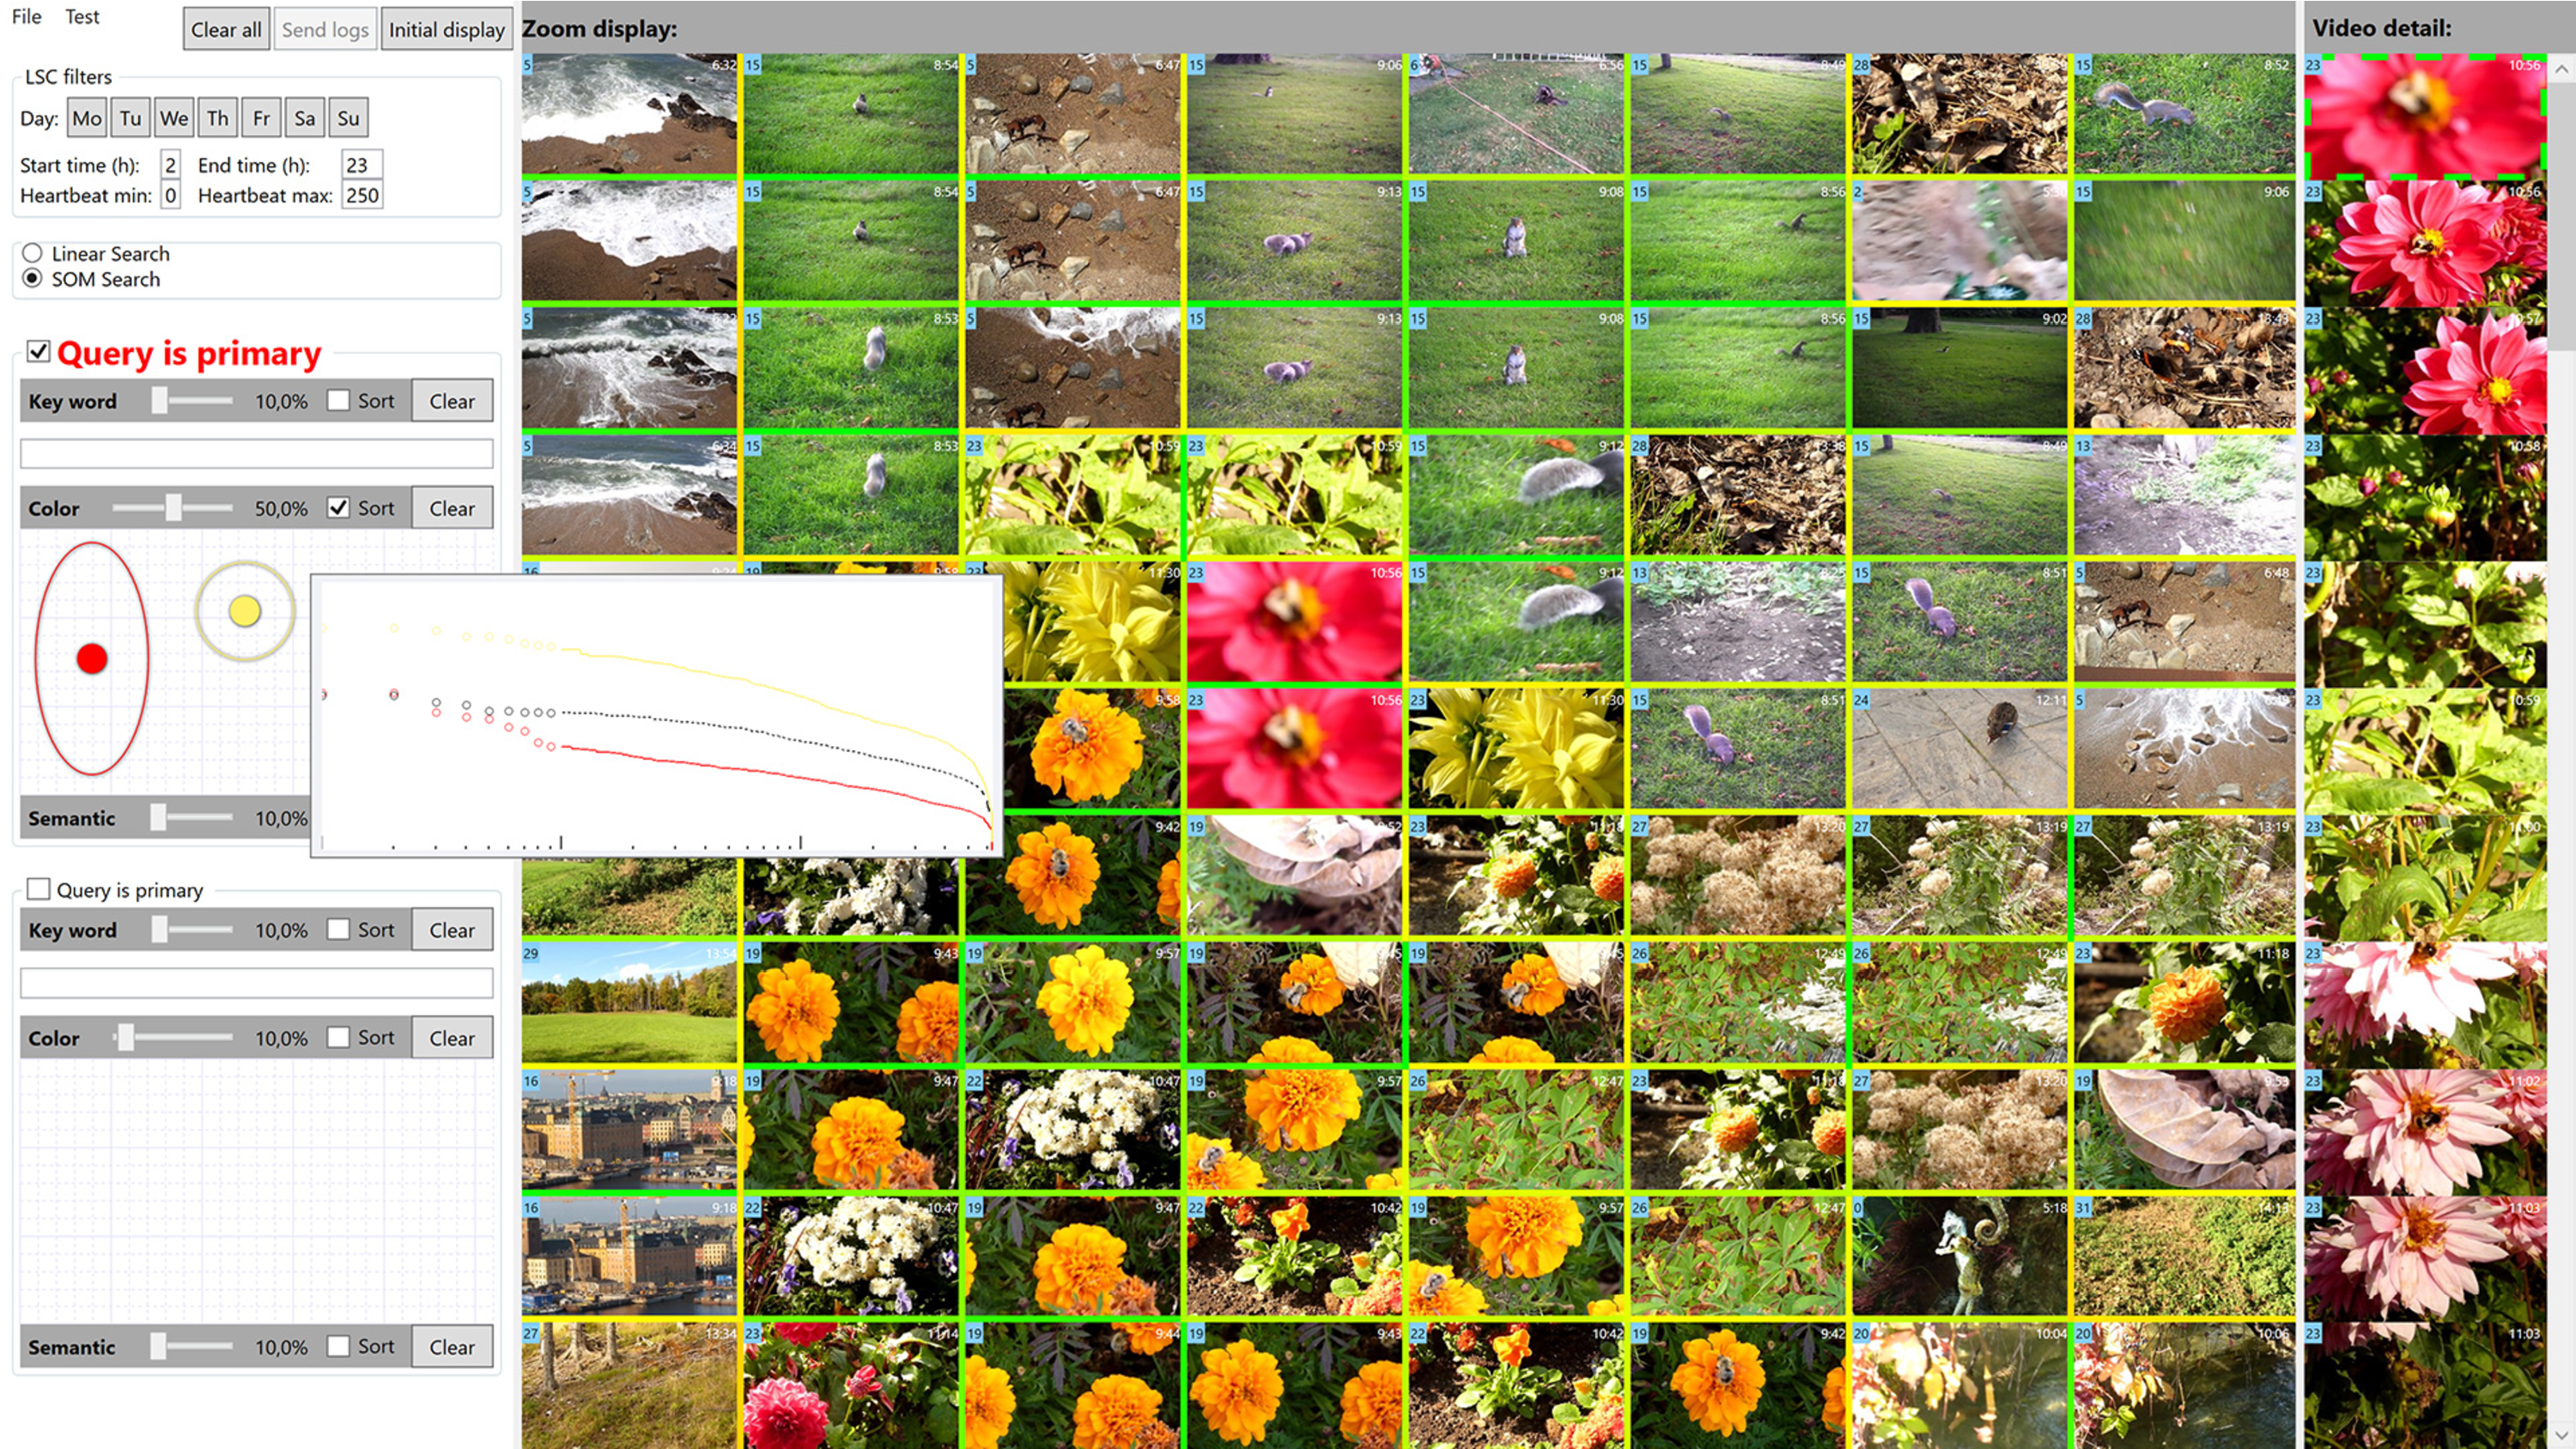
\includegraphics[width=\linewidth]{img/viret_overview.pdf}
    \caption[Example search in VIRET framework]{Example search in VIRET framework. Source: \cite{kovalvcik2020viret}}
    \label{fig:viret}
\end{figure}

\subsection{SOM-Hunter}

A SOM-Hunter was for the first time introduced at the \acrshort{vbs}2020. This tool is related to our approach because it also supports Self-organizing Maps to solve a Known-item-search task. The typical workflow (as described in \cite{kratochvil2020som}) starts with a search based on the keywords. This reduces the dataset only to relevant images. During the entire browsing session, they preserve the relevance score for each image. To display the results, they use a mapping onto a trained self-organizing map weighted by the relevance scores or a grid view sorted by the relevance scores. The user can continue to explore the dataset further by browsing or reformulating the query. Since the showed displays are relatively small ($8\times8$ images when using a \acrshort{som}), the corresponding self-organizing map can be computed quickly. The user can also explore the temporal context of any of the images. A sample interaction with the system is displayed in \autoref{fig:som_hunter}.


\begin{figure}
    \centering
    \includegraphics[width=0.99\linewidth]{img/som_hunter_small.png}
    \caption[A sample search in SOM-Hunter]{A sample search in SOM-Hunter. Source: \href{https://videobrowsershowdown.org/hall-of-fame/}{Video Broser Showdown, Hall of Fame}}
    \label{fig:som_hunter}
\end{figure}

\subsection{Vitrivr}

Vitrivr [\cite{rossetto2016vitrivr}, \autoref{fig:vitrivr}] is a sophisticated framework for retrieving a video in the collection. Vitrivr is separated into three modules, Vitrivr-ng, Cineast, and Cottontail-DB.  Vitrivr-ng is the module responsible for creating queries that are later processed by the Cineast. Cottontail-DB supports fast retrieving methods of the features required by Cineast. The overview of the system is displayed in figure \ref{fig:vitrivr}. Vitrivr supports different query types: query by a sketch, as well as an example image, semantic concept, keywords, audio, or motion. The feature extraction and the system behind retrieving the most similar results are parts of the second module -- Cineast (\cite{rossetto2016searching}). Cineast uses multiple approaches incorporating deep features, e.g., scene text recognition and speech-to-text recognition. Vitrivr-ng (the part responsible for creating the queries) is a web-based software. The modules structure provides a clean separation between the query formulation and feature extractions.

\begin{figure}
    \centering
    \includegraphics[width=\linewidth]{img/vitrivr.png}
    \caption[Overview of the separation in the Vitrivr framework]{Overview of the separation in the Vitrivr framework. Source: \url{https://vitrivr.org/vitrivr.html}}
    \label{fig:vitrivr}
\end{figure}

\section{Face Recognition}

In the second part of the thesis, our goal is to organize faces to allow a faster search through the dataset. We leverage the face recognition technology to organize the faces into a hierarchical structure. One such approach is presented in \citep{girgensohn2004leveraging}. The authors' algorithm provides users with faces based on the similarity to existing models (i.e., person). They examined the performance of the model by a series of simulations. 

In recent years, many steps have been taken towards solving the face recognition task. As the \cite{ranjan2018deep} overviews, three separable modules are typically needed for automatic verification and identification systems. Firstly, a face detector is applied to localize faces in images. A robust detector should be able to detect faces with a varying pose, illumination, and scale. Also, the bounding boxes of the detected faces should be minimized, to contain a minimal amount of background. Secondly, a landmark detector is usually incorporated. This detector localizes the important facial landmarks such as nose tip, mouth corners, etc. These points are then used to rotate and scale the face, which creates a normalized input for the next phase. Lastly, a feature descriptor encodes information from the aligned face. Based on these encodings and various similarity measures, the model can signify if the two faces belong to the same person or perform other related tasks.

The face recognition problem can be further split into two categories: face verification and face identification. In the face verification task, the goal is to determine whether two subjected faces belong to the same person. In the identification scenario,
a set of known subjects is inserted into the system. Then, a new subject (target) is presented. The goal of the model is to retrieve all faces from the dataset belonging to this person, or in a supervised manner, to assign the identity.

Since the early 1990s, many face identification/verification systems were proposed. For example, in \citep{kalocsai1998face}, authors conducted a study, where two faces were shown to the respondents, simulating the verification task. Then, the respondents were asked to decide if the faces belong to the same person. The faces displayed different emotions. The researchers suggest that the model's performance correlates with the subjective human representation of the faces.

Twenty-five years later, with the advancements of the deep neural networks, new state-of-art methods achieve an almost perfect score on some of the benchmarks (e.g., \citep{huang2008labeled}). We refer to the \citep{masi2018deep} to provide an overview of the recent models used for face identification and verification. The summary also provides a thorough description of the individual steps usually taken by the approaches presented. In our work, we use pre-trained models provided by the dlib library. We include more technical information in section \ref{s:dlib}.

\section{Dataset}
\label{s:dataset}

We use Vimeo Creative Commons Collections (V3C1)\footnote{\href{https://www-nlpir.nist.gov/projects/tv2019/data.html}{TRECVID 2019 Video Data}} dataset for experimenting and evaluations. This dataset is used for evaluations at \acrshort{vbs} and also at TRECVID. The dataset is composed of 7475 Vimeo videos. We selected only the first 750 videos for proving concepts of our work. From these 750 videos, 111\ 764 images were extracted with resolution 320x180 by using an extraction tool from \cite{lokovc2019framework}. I extend my gratitude to Tomáš Souček and Gregor Kovačík for providing extracted images.

The videos capture a wide range of sceneries on many different occasions. We can see many different landscapes, from seas to mountain views, from desert to snow. A large proportion of the videos contain people. Videos capture people doing different activities, e.g., Hindi wedding, skateboarding in a park, or a news broadcast.


\chapter{Theoretical and Technical Background}
\label{ch:technical_background}

This chapter intends to review the fundamentals of the theoretical approaches used in this thesis. It includes the fundamental concepts of neural networks and a short description of the networks we use. The chapter also reviews projection methods of high-dimensional data to lower-dimensional space.

\section{Deep Neural Networks}

In recent years we witnessed the emergence of many records-breaking machine learning models. Many of those breakthroughs were possible, thanks to the advancement of Deep Neural Networks (\acrshort{dnn}). Nowadays, these models replaced more traditional Machine Learning approaches in many tasks.

Deep Neural Network is a machine learning model, whose goal is to approximate a given function \(f\). The set of its parameters is often referred to as \(\theta\). One of the everyday tasks performed by these networks is classification, where the goal of the network is to predict which category sample \(X\) belongs to. Even though we will not perform a classification task in this thesis, we will use some of the available classification networks.

When we talk about neural networks, we usually refer to a feedforward network. These networks consist of layers that only pass information in one direction during the evaluation. We can imagine it as applying a function to the results from the previous layer. For example, let us create a small neural network. Denote first layer as \(f_1\) and second layer as \(f_2\). The output of the network will be \(f_2\left(f_1\left(\cdot\right)\right)\).

Stacking more and more layers on top of each other leads us to the notation \emph{deep} neural networks. This notation has no fixed threshold on which networks ``deserve'' to be called deep. The word ``deep'' separates the eras between the neural networks consisting of a couple of layers from neural networks consisting of tens or more layers.  

The first and last layers are commonly referenced as an \emph{input} and \emph{output} layer, respectively. Layers between the input and output layers are usually denoted as \emph{hidden} layers. Deep neural networks can have four or hundreds of layers, and there are multiple types of operations that the layer can perform. \emph{Network Architecture} captures the ``build order'' of the network. It is important to note that there exist many networks with different architectures solving the same task.

There are many reasons for the advancement of neural networks in the past years. One of the crucial stones was not only theoretical innovations used for the networks but increasing computability limits. Deep Neural Networks \emph{learn} to approximate function by \emph{training}. This training is usually the heaviest part of the computation. Even though it is enough to train it once and use it forever, it usually lays some limitations on the size of the networks or the functions used.

Since this topic is broad, we recommend more thorough reading, such as Neural Networks and Deep learning online book \citep{nielsen2015neural}.

\subsection{Convolution Neural Networks}

Convolution Neural Networks (\acrshort{cnn}) are a class of Deep Neural Networks. Even though they emerged in the late 1980s \citep{lecun1989backpropagation}, it took another 20 years for further advancements in the research area. Convolution Neural Networks are mainly used in image-related tasks, such as image classification (``What is on the image?''), object detection (``Where are the objects in the image and what are they?'') or even content generation (``Create a new image''). Their abilities were also tested in many, not image-related tasks, e.g., music genre recognition.

Convolutional Neural Networks are specialized kind of networks which usually work with grid-like topology. For the 2D case, most typically image pixels represent a grid. The name \emph{convolution} refers to using a mathematical linear function \emph{convolution} in at least one of the layers. A simplified overview of the structure is displayed in figure \ref{fig:convolution_neural_network}. We refer to \cite{Goodfellow-et-al-2016} for additional information about the \emph{convolutional layers}.

\begin{figure}
    \centering
    \includegraphics[width=0.98\textwidth]{img/convolution_neural_network.jpg}
    \caption[Schematic diagram of a convolutional neural network]{Schematic diagram of a convolutional neural network. Source: Phung, V.H.; Rhee, E.J. A High-Accuracy Model Average Ensemble of Convolutional Neural Networks for Classification of Cloud Image Patches on Small Datasets. Appl. Sci. 2019, 9, 4500.}
    \label{fig:convolution_neural_network}
\end{figure}

\subsection{Transfer Learning}

Transfer Learning is a research problem in machine learning that focuses on storing knowledge gained while solving one problem and applying it to a different problem. We have seen many successful transfers of the network architecture and parameters learned to a new task. Transfer learning may help to reduce the cost of the training and often also to overcome an insufficient set of training examples for the new task.

We utilize some of the pre-trained Convolution Neural Networks. The possibility of using a pre-trained neural network on a different task than they were trained on was explored as early as 2014 by \cite{donahuedeep}, and many others were able to use this process to acquire better models.  Networks we use are mostly pre-trained on \emph{ImageNet}\footnote{http://www.image-net.org/}. ImageNet serves as one of the benchmarks for comparing the performance of the different networks. Since the ImageNet Challenge is a classification task, we utilize the transfer learning to obtain deep features, by stripping the last classification layer. Layers at the end of the networks accumulate semantic information, i.e., they contain high-level features. Therefore, we work with the layers close to the output layer. These layers represent encoded information about the image in high dimensional vectors. Our task is to use these deep features obtained for solving our known-item search task.

\begin{figure}
    \centering
	\includegraphics[width=0.8\linewidth]{img/network-comparison.jpeg}
	\caption[Top-1 one-crop accuracy versus amount of operations required for a single forward pass]{Top-1 one-crop accuracy versus amount of operations required for a single forward pass. The size of the blobs is proportional to the number of network parameters. Source: \cite{canziani2016analysis}}
	\label{fig:camera-setup}
\end{figure}

\subsection{Pretrained models}
\label{ss:pretrained_models}

In our work, we use various pre-trained models. We obtain the models from Keras, dlib, or other open-sourced projects. In the following sections, we describe the frameworks and libraries we use.

\subsection{Keras}

Keras \citep{chollet2015keras} is a deep learning \acrshort{api} written in Python, running on top of the machine learning platform TensorFlow \citep{tensorflow2015-whitepaper}. It was developed with a focus on experimentation in deep learning. We use it and its pre-trained models in this thesis. The models, which we use from Keras Applications, were trained on ImageNet. Keras API allows us to remove the last fully connected layer used for classification (since default ImageNet is a classification task) from the selected neural network.

In this thesis, we use pre-trained models to implement new approaches. We do not aim to train new models or further train existing ones. We try to extract the information from available models to solve the known-item search task. Here we describe two models which we experimented with the most. ResNet was a state of the art model as of 2015. Since then, it gained popularity in many tasks. The second network we focus on is MobileNet. MobileNet has excellent performance to complexity ratio. Therefore, it is an ideal network for our purpose, where the predictions need to be computed online and displayed to the user.

\subsection*{Resnet50V2}

ResNet (abbv. for Residual Networks, \cite{resnet}) is a classic neural network used in many computer vision tasks. ResNet was the winner of the ILSVRC 2015 (\citep{ILSVRC15}). The authors aimed to solve the problem of degrading the training accuracy of the neural networks when more layers were added. 

The authors argued that the reason behind the degradation is that approximating identity function by a layer in a neural network is difficult (otherwise, the added layers should learn to approximate identity, and the resulting error should be no greater than when using shallower counterpart). To solve this problem, instead of trying to approximate underlying mapping $H(x)$, they ask the neural network to approximate residual function $F(x)=H(x) - x$. That way if identify is suitable function the weights just needed to be driven to zero (achieve $0 = H(x) - x$ i.e. $H(x) = x$). They do so by replacing simple layers by residual building blocks (see figure \ref{fig:resnetv2}).

\begin{figure}
    \centering
    \includegraphics[width=0.5\textwidth]{img/resnetv2.png}
    \caption[Residual units]{Left: ResNet residual unit as proposed in \citep{resnet}. Right: ResNetV2 residual unit by \citep{resnetv2}. Source: \cite{resnetv2}}
    \label{fig:resnetv2}
\end{figure}

In \citep{resnetv2}, the authors improved the architecture of ResNet by changing the position of activation a batch normalization layers. By doing so, they made the easiest path for the information to propagate even simpler. For details see the figure \ref{fig:resnetv2}. This improved architecture is commonly known as ResNetV2.

\subsubsection*{MobileNetV2}

In April 2017, a group of researchers from Google published a study \citep{mobilenet} introducing a new neural network architecture. This MobileNet was optimized for mobile devices. They optimized the model to deliver high accuracy while keeping the model and mathematical operations as fast as possible. Not a year later, MobileNetV2 was introduced by \cite{mobilenetv2}. It extended the predecessor by using Inverted Residuals with Linear Bottlenecks. For more details, please refer to the original research. In our work, we use only MobileNetV2 out of MobileNets.


\subsection{Dlib}
\label{s:dlib}

Dlib \citep{king2009dlib} is a modern C++ toolkit containing machine learning algorithms and tools for creating complex software in C++ to solve real-world problems. We use the Dlib library for face detection and also face feature extraction. For both, we use Python \acrshort{api} provided by \verb+face_recognition+ \citep{geitgey2016machine}. 

\subsubsection*{Face detection}

The authors of dlib implemented two key approaches to face detection. The first one, the frontal face detector, is based on the histogram of gradients. This approach is very fast in learning to detect the faces and also fast on performing the detections. It is still used in a variety of online tasks. The original release notes are available in \citep{king2017dlib_hog}.

The second approach present in the dlib is based on the convolutional neural network. This approach has a longer inference time. However, based on evaluations, it has higher accuracy in non-frontal face views. The overview of both approaches is provided, for example, by \citep{arun2018cnndlib}.

\subsubsection*{Face encodings}

Dlib also presents a model for face encoding extraction. This model was trained for the face verification task. Based on published results (\href{http://vis-www.cs.umass.edu/lfw/results.html}{Labeled Faces in the Wild Benchmark}), the model achieves  99.38\% accuracy on the verification task. The network architecture is based on the ResNet34 and trained on the mix of the available datasets of faces. The review of the model is available at \citep{king2017high}.

\section{Principal Component Analysis}
\label{s:pca}

In projection methods for dimensionality reduction, the goal is to find a mapping of the input vectors from the original $d$-dimensional space to a new $k$-dimensional space (where $k < d$) with minimum information loss. \acrshort{pca} is one of such methods. It is an unsupervised method, which employs linear projection to decrease the number of dimensions while preserving the explanation for variance within the data. Since the derivation of the formulas for \acrshort{pca} requires several technicals steps and some advanced knowledge of Linear Algebra, we refer to the \cite{alpaydin2020introduction} for a more detailed description.

\section{Self-organizing maps}
\label{s:som}

The self-organizing map was introduced by \cite{kohonen1982self}. The self-organizing map, abbreviated as \acrshort{som}, is an example of a popular neural network based on unsupervised learning.  It produces low-dimension (typically two-dimension), discretized representation of the input space. Additionally, the \acrlong{som} structure forms a semantic map, where similar samples are mapped close together and dissimilar ones further apart.

The SOM consists of neurons $M$ organized on a regular low-dimensional grid. Each neuron is represented by a $d$-dimensional weight vector, where $d$ is equal to the dimension of the input vectors, we shall denote this mapping $\phi: M \rightarrow \mathbb{R}^d$. Each neuron is connected to the adjacent neurons by a neighborhood relation, which is induced by the distance between their representations in the low-dimensional space and a threshold. This relation creates the structure of the map. 

During the training, the weight vectors are initialized with random values. Then, iteratively, we find the closest weight vector to a data point, called the Best Matching Unit (we denote such mapping $\mu: \mathbb{R}^d \rightarrow M$). We shift the weight vector of the \acrshort{bmu}, and usually also weight vectors of the neighboring neurons, closer to the data point. The impact on the neighboring neurons is usually scaled by the distance from the BMU.

The SOM can be thought of as net spread across the data. After the training, the neighboring neurons on the grid get similar weight vectors. For a more detailed description, please refer to \cite{kohonen1982self} and \cite{kohonen2007kohonen}. Extensive research on the topic of image retrieval using SOM was also presented by \cite{koskela2003interactive}.

Various measures have been developed to quantify a map's quality. In this thesis, we use the following two: quantization error and topographic error. For the motivation behind the errors and more information about them, we refer to \cite{breard2017evaluating} and the original research. Here we present their definition and brief description.

\subsubsection*{Quantization Error}

A quantization error is formulated, for example, in \cite{wandeto2019quantization}. It is a measure of the average distance between the data points $x_i \in X$ and the map nodes to which they are mapped. The quantization error $QE$ for a map $M$ is calculated as follows:

$$
 QE(M) = \frac{1}{n}\sum_{i=0}^{n-1} ||\phi(\mu(x_i)) - x_i ||
$$

where $n$ is the number of samples in the training data $D$.

\subsubsection*{Topographic Error}

The topographic error was introduced by \cite{kiviluoto1996topology}. It accounts for a SOM's ability to preserve local topological features in low dimensional output space. A sample for which the best matching unit and the second-best matching unit are not adjacent counts as an error. The topographic error is given by the total number of errors divided by the total of samples.

$$
    TE(M) = \frac{1}{n}\sum_{i=0}^{n-1}t(x_i)
$$

$$
    t(x) = \begin{cases}
			0, & \text{if $\mu(x)$ and $\mu'(x)$ are neighbors}\\
            1, & \text{otherwise}
		 \end{cases}
$$

where $\mu'(x)$ returns the second-best-matching unit.
\chapter{Content-based image retrieval}
\label{ch:preliminaries}

Image retrieval and image indexing have been an active research field since the 1970s. In 1978 (\cite{tamura1978textural}), a group of researchers proposed a system for retrieving textures based on the example texture. Since then, a wide range of techniques for image retrieval were presented. Traditional approaches included manual annotation of the images by textual or numerical metadata. The user could then formulate a query against these annotations to retrieve relevant images. This approach is often referred to as Concept-based image retrieval or meta-data search.

There are several drawbacks to the textual or numerical annotations. First of all, extensive human annotations are often needed to provide rich data for filtering. Including also, spatial information of the objects takes more resources than only writing down present objects in the image. Furthermore, the images often include too many details (i.e., type, color, or shape of the objects), which may be impossible to comprehend by manual annotations.  The annotations may not even represent a stable truth. With a different annotator, the annotations may include different details/objects, which were perceived differently. When the user searches for an image, she has to know the exact terms the annotators used in order to be able to retrieve the images they want. As the last problem, we pose with human annotations is the scalability. As the amount of information increases every second, there is no human capability to hand process all the examples.

During the 1990s, content-based image retrieval (CBIR) emerged (trend study from \cite{datta2008image}). In the CBIR approach, the images are indexed by features directly derived from their visual content using automatic or semi-automatic image processing techniques. Such indexing lacks building blocks (for example, verbal description); on the other hand, it provides low-level feature information about the whole images or its regions. The attributes of images are complex functions of regions of the image or the whole image.

CBIR has received considerable research interest in the last decades. With the advancement in Deep Learning, a new pool of possible complex functions to describe the images emerged. In our approaches, we use pre-trained neural networks to extract features. Based on these features, we implemented and evaluated several approaches to the CBIR task.

Presented techniques focus on the known-item search task. An alternative could be an Ad Hoc search, where the goal is to retrieve all relevant items to the query. Known-item search task instead works with retrieving a known item from the dataset.

Following this chapter, we continue with the specifics of the individual approaches we present. Here we formulate the task and the goal.






\section{Task formulation}
\label{s:task_formulation_preliminaries}

The goal of the thesis is to propose a system that can search and retrieve images based on visual similarity.  

First we define universe $\mathcal{U}$ as the set of the all possible images:

$$
    \mathcal{U} = \bigcup_{h,w \in \mathbb{N}^2} \{0, 1, 2, \ldots 255 \}^{h \times w \times 3}
$$

This definition follows the standard description of an image as a matrix $w \times h$ of pixels, where three color channels describe each pixel. We work over a dataset $D$ of such images, that we can define as $D \in \mathcal{P(U)}$.

The user is then presented with a target image $T \in D$ and asked to locate the image within the dataset $D$. This task is called a known-item search. 

Our system then serves as a search engine, aiming to provide the user with the most relevant results based on the user input. The system leverages the visual similarity between the images in the dataset $D$ (as in chapter \ref{ch:face_search}), or the similarity between user-provided example pictures and the images from the dataset $D$ (as in chapter \ref{ch:object_location}).

\section{Feature space}

To search over a dataset of images $D$, we need a metric of how similar two items are. This similarity could be computed between the images directly, although it is more common to compare two images after a projection by a descriptor. A descriptor is a function $f_e: \mathcal{U} \rightarrow \mathcal{R}$, where $\mathcal{R}$ is a representation universe. Given a descriptor $f_e$, we compute for each image in the dataset $D$ a feature vector $L_I = f_e(I)$, where $I \in \mathcal{U}, L_I \in \mathcal{R}$. In our work, we use various neural networks as our descriptors. It is common for neural networks to produce the representations in the space of real numbers $\mathbb{R}^n$, and in our case, we work only with the representation spaces, which are isomorph to the $\mathbb{R}^n$.

\section{Distance Measures}

To compare, how similar representations of two images are, we use a concept of distance. Similar representations have smaller distance, and vice versa. We use a definition for a distance space and metric space from the book \cite{deza2009encyclopedia}.

\theoremstyle{definition}
\begin{definition}{Distance space}
$(\mathcal{U}, \delta )$ is a set $\mathcal{U}$ equipped
with a distance $\delta : \mathcal{U} \times \mathcal{U} \rightarrow \mathbb{R}^+ \text{ satisfying } \forall x, y \in \mathcal{U}: \delta(x, y) \geq 0 \text{ (nonnegativity), } \delta(x, y) = \delta(y, x) \text{ (symmetry) and } \delta(x, x) = 0.$
\end{definition}

\theoremstyle{definition}
\begin{definition}{Metric space}
$(\mathcal{U}, \delta)$ is a distance space, where $\delta$ additionaly satisfies $\forall x, y, z \in \mathcal{U} : \delta(x,z) \leq \delta(x,y) + \delta(y,z)$ (triangle inequality) and $\delta(x, y) = 0 \Rightarrow x = y$
\end{definition}

In the next chapters, we often compare two high-dimensional feature vectors. These vectors are often produced as a prediction of a neural network. Our feature space is $\mathbb{R}^n$, given $n$ as the number of features. We search for a distance measure function $d: \mathbb{R}^n \times \mathbb{R}^n \rightarrow \mathbb{R}$. We use the following three:

Here we present distances over the space $\mathbb{R}^n$ later used in the thesis. Euclidean and Manhattan distances on $\mathbb{R}^n$ are metrics spaces. Cosine distance, deduced from cosine similarity does not follow triangle inequality and forms only a distance space.

\subsection{Euclidean distance}

For given $\bf{p}, \bf{q} \in \mathbb{R}^n$ we compute the distance as:
\begin{equation}
d_e({\bf p},{\bf q}) = \sqrt{\sum_{i=1}^n (p_i - q_i)^2}    
\end{equation}


\subsection{Manhattan distance}

For given $\bf{p}, \bf{q} \in \mathbb{R}^n$ we compute the distance as:
\begin{equation}
d_m({\bf p},{\bf q}) = {\sum_{i=1}^n |p_i - q_i|}    
\end{equation}


\subsection{Cosine similarity}

For given $\bf{p}, \bf{q} \in \mathbb{R}^n$ we compute the similarity as:
\begin{equation}
\text{similarity}({\bf p},{\bf q}) = \cos ({\bf p},{\bf q})= {{\bf p} {\bf q} \over \|{\bf p}\| \|{\bf q}\|} = \frac{ \sum_{i=1}^{n}{p_i q_i} }{ \sqrt{\sum_{i=1}^{n}{p_i^2}} \sqrt{\sum_{i=1}^{n}{q_i^2}} }
\end{equation}

Since the cosine similarity is bounded by one, we use a transformation $d = 1 - s$ to obtain a distance.

\begin{equation}
    d_{cos}({\bf p},{\bf q}) = 1 - \text{similarity}({\bf p},{\bf q})
\end{equation}
% \chapter{Content-based image retrieval}
\label{ch:content_based}

Image retrieval and image indexing has been an active research field since the 1970s. In the 1978 (\cite{tamura1978textural}) a group of researchers proposed a system for retrieving textures based on the example texture. Since then, a wide range of techniques for image retrieval were presented. Traditional approaches included manual annotation of the images by textual or numerical metadata. The user could then formulate a query against these annotations to retrieve relevant images. This approach is often referred to as Concept-based image retrieval or meta-data search.

There are several drawbacks to the textual or numerical annotations. First of all, extensive human annotations are often needed to provide rich data for filtering. Including also spatial information of the objects takes more resources than only writing down present objects in the image. Furthermore, the images often include too many details (i.e. type, color, or shape of the objects), which may be impossible to comprehend by manual annotations.  The annotations may not even represent a stable truth. With a different annotator, the annotations may include different details/objects, which were perceived differently. When user searches for an image, they have to know the exact terms the annotators used in order to be able to retrieve the images they want. As the last problem, we pose with human annotations is the scalability. As the amount of information increases every second, there is no human capability to hand process all the examples.

During the 1990s, content-based image retrieval (CBIR) emerged (trend study from \cite{datta2008image}). In the CBIR approach, the images are indexed by features directly derived from their visual content using automatic or semi-automatic image processing techniques. Such indexing lacks building blocks (for example verbal description), on the other hand, provides low-level feature information about the whole images or its regions. The attributes of images are complex functions of regions of the image or the whole image.

CBIR has received considerable research interest in the last decades. With the advancement in Deep Learning, a new pool of possible complex functions to describe the images emerged. In our approaches, we use pre-trained neural networks to extract features. Based on these features, we implemented and evaluated several approaches to the CBIR task.

Presented techniques focus on the \acrlong{kis} task. An alternative could be an Ad Hoc search, where the goal is to retrieve all relevant items to the query. Known-item search task rather works with retrieving a known item from the dataset.

Following this chapter, we continue with specifics of the individual approaches, we present. Here we formulate the task and the goal.

\section*{Task formulation and evaluation}

As our inputs we have a dataset of images and the target image (the image we look for). Since we work with known-item search task, we know that a target image is also present in the dataset. Our goal is to order the items in the database in a way, that the target image has the lowest rank. Alternatively said, if we order based on the similarity, we aim for the query and the target image to have the highest similarity. We refer to the position of our target image $t$ in ranked results as $rank_t$.
\todo[inline]{pozice obrazku v tomto usporadani je rank t vzhledem ku q je tolko}
\todo[inline]{we aim fot the query to have the highest similarity with the target image, good rank}
\todo[inlline]{v grafe, na x ovu os dat rank, popisat rank ... }
\todo[inlline]{\% of searched target images up to a given rank}
\todo[inline]{pripominame ze pozia obrazku v usporiadani oznacujeme ako rank}

Our goal is to develop a technique, which minimises the rank of the target image. In the following chapters we aim to test two different possibilities for query description.

We also provide a numerical comparison of the performance of different setups. To provide a comparison we a \emph{Rank of searched item}. The graphs shows the amount of the queries solved in a given rank. In all graphs an x-axis \todo{jednotky databaze a rank is represented as a percentage of the dataset} . The amount of queries solved is also expressed as the percentage.

\todo[inline]{nedava zmysel ten odstavec, krivka vyznacuje nie obsahuje, oznacuje mnozstvo dotazov up to a given rank}


We use a figure \ref{fig:mobilenet_whole_image_example} as an example to explain the graphs we use for evaluation of the performance of the system. In this specific case for 90\% of the annotated collages (queries), the target image was ranked in the first 50\% of the dataset. This can be also said in other words, that in 90\% of cases by stating a query we were able to eliminate half of the dataset as unrelated. We can also notice a steep curve in the beginning. It shows that 70\% of the collages had the target image ranked in the first 10\% of the dataset. We can see that this particular system worked well for 70\% of the collages well, but struggled to solve the rest.

\begin{figure}
    \centering
    \includegraphics[width=0.8\linewidth]{img/mobilenet_whole_image.png}
    \caption{Performance of MobileNetV2 on annotated collages}
    \label{fig:mobilenet_whole_image_example}
\end{figure}

For these evaluations we use annotated queries. We described them in the section \ref{s:dataset}.
\chapter{Search by Object Location}
\label{ch:object_location}

% \todo[inline]{v grafe, na x ovu os dat rank}
% \todo[inline]{\% of searched target images up to a given rank}

\normalem
\emph{You see a picture in your head. Your friend is standing on the beach, and there is a little sandcastle on the left. The sea behind beautifully reflects the sun, which is setting.}
\ULforem

We can imagine that at that particular moment we were shooting a video of the scenery. However, years later, with a vast set of videos in our collections, it may be impossible to re-watch every one of them to find that particular memory. Not all of us can visualize the memory, but about those who can, we say that they have an excellent visual memory \footnote{\url{https://en.wikipedia.org/wiki/Visual_memory}}. We present a technique that can be used to search in a dataset based on such memories of the scenery.

In this chapter, we elaborate approaches for known-item search task based on the visual description of the image. The input is characterized by the way how the objects looked (by providing example images) and their relative location in the image (i.e., top left corner). With that information, we look for a match in the database to the described image. We refer to our input as \emph{collage query}, or simply just as a collage. Collage is created by taking images and placing them onto an empty canvas. The placement of the images also carries a piece of information. We show an example of such a collage (query) in figure \ref{fig:query_collage_comparison}. On the left, we can see a cat in the center behind a window. On the right, we can see a possible visualization of such memory. On the grey canvas, we placed a window, which reminded us of the original one. At the center, we added a similarly colored cat.

\begin{figure}
\centering

\begin{subfigure}[t]{0.45\textwidth}
\includegraphics[width=0.9\linewidth]{img/cat_on_window} 
\caption{Target image}
\label{fig:searched_scene}
\end{subfigure}
\begin{subfigure}[t]{0.45\textwidth}
\includegraphics[width=0.9\linewidth]{img/cat_on_window_collage}
\caption{One of the possible collage description of the target image}
\label{fig:collage_example}
\end{subfigure}

\caption{Example of searched image (target) with possible visual description by a collage.}
\label{fig:query_collage_comparison}
\end{figure}

While we were describing the image, we used words for it. However, in this chapter, we do not focus on the search based on the verbal description of the objects. Compared to such a textual approach, we can capture more diversity in the objects by visual information. For example, a single word for a human may represent a visually wide range of possibilities based on clothes, age, and other attributes. On the other hand, these attributes are easier to capture by providing an example image.


This chapter will present three approaches incorporating pre-trained neural networks. We start with the formalization of the task. Next, we provide a short description of user-program interaction and a description of the annotated queries used for evaluations. We use this annotated set of queries to test different sets of hyperparameters and investigate their effect on the system's performance.

\section{Formal description}

In this task we explore the dataset $D$ based on the collage provided by the user. We shall formally define universe of query images as follows: 
$$
    \mathcal{Q} = \{(I, x_0, x_1, y_0, y_1) | I \in \mathcal{U}, x_0 \in [0,1), y_0 \in [0, 1), x_1 \in (x_0, 1], y_1 \in (y_0, 1] \}
$$
where $\mathcal{U}$ is a universe defined in section \ref{s:task_formulation_preliminaries}. $I$ represents an image in the collage; $x_0$, $y_0$ represent the relative position of the top left corner of the image in the canvas; $x_1$, $y_1$ represent the relative position of the bottom right corner of the image in the canvas. Single collage $Q$ is then defined as $Q \subset \mathcal{Q}$

Ultimately, we would like to construct a function $r^*$, that for each query $Q_i \subset \mathcal{Q}$ would find corresponding target image $T_i \in D$. Formally, we can define this function as follows:
$$
    r^*: \mathcal{P(Q)} \rightarrow D 
$$
$$
    r^*(Q_i) = T_i \, \forall (Q_i, T_i) \in X
$$
where $X$ is a set of target images and corresponding queries constructed by the user.

However, due to imperfect user queries, this task maybe even impossible. Therefore, we focus on reordering the dataset, in the way that linear search by the user in this order would provide the target image as quickly as possible. We define \emph{ranking} $r_{D, Q}$ as function with respect to a given dataset $D$:
$$
    r_D: (D \times \mathcal{P(Q)}) \rightarrow \{0, 1, \ldots |D|-1  \}
$$
$$
    \text{ s.t. } \{r_D(d, Q) | d \in D \} = \{0, 1, \ldots |D|-1  \} \, \forall Q \subset \mathcal{Q}
$$

In other words, $r_D(T, Q) = n$ means that target image $T$ is in position $n$ after ordering the dataset $D$ with respect to collage $Q$. This value correlates with the time spend on the linear search of the provided ordered results. This gives us the motivation to evaluate our algorithm based on this \emph{rank} across the whole set $X$.



\section{User-program interaction}

We provide a user with a canvas where they can place, move, and resize the collage images. They can add images by providing an URL of the image, or by pasting the image from a clipboard. One possible way to obtain images for the collage is to use an image search engine (e.g., Google Images). The images can be usually copied to the clipboard by selecting copy in the right-click menu. A quicker approach, we preferred, is using selective screenshots. With the selective screenshot, we can even crop the image, focusing on the part we like, and paste it onto the canvas.

Based on the provided collage, the program searches for similar images in the dataset and interactively presents them back to the user. The user can then alternate the query for a new search, or investigate the displayed results. Figure \ref{fig:query_collage_comparison} shows an example of the query -- the collage of two images (window and cat). 

\subsection{Collected collages}

We manually created a set of queries to evaluate the proposed systems. The annotated data consists of 102 collages, each containing a visual description of a given target image. The average size of the images used in the collages covers 15\% of the canvas. Five percent of the dataset consists of images bigger than 80\% of the canvas. We provide visualizations of the distribution of the annotated queries in figure \ref{fig:annotated_dataset}. Together, all 102 collages are annotated by 199 images.

\begin{figure}
     \centering
     \begin{subfigure}[b]{0.48\textwidth}
         \centering
         \includegraphics[width=\textwidth]{graphs/num_queries_in_request.pdf}
         \caption{Number of images on a canvas for a collage.}
         \label{fig:y equals x}
     \end{subfigure}
     \hfill
     \begin{subfigure}[b]{0.48\textwidth}
         \centering
         \includegraphics[width=\textwidth]{graphs/queries_size.pdf}
         \caption{Size of the canvas which is covered by a query image.}
         \label{fig:three sin x}
     \end{subfigure}
    
    \caption{Annotated collages properties}
    \label{fig:annotated_dataset}
\end{figure}

For the annotation, we used our application. It is possible to save the collage by clicking ``Submit Collage.'' The average time spent on creating a single collage was 91 seconds. This time includes searching for images online, pasting them onto the canvas, and usually also waiting for the responses of the system.

We want to highlight that we created more than a hundred collages corresponding to the target images from the dataset. The annotations were done only by a one-person. We leave annotation from more people, to study the differences in behavior, for future work. 

\section{Framework overview}

\begin{figure}[p!]
    \centering
    \includegraphics[scale=0.9]{img/features_pipeline.png}
    \caption{Overview of processing pipeline}
    \label{fig:processing_pipeline}
\end{figure}

Our approach consists of several individual steps. Figure \ref{fig:processing_pipeline} shows a visual overview of the steps we describe here. Our first step is to compute feature vectors for each image, given the descriptor. We call this step \emph{feature extraction}. This way, we obtain \emph{records}, i.e., a pair of image from the dataset and its corresponding feature vector. In the figure, we show the possibility of having multiple feature vectors in the same record. Using multiple feature vectors is still following our theoretical model since the space from the concatenation of the feature vectors is isomorph to the $\mathbb{R}^n$. Therefore, we can still think of it as one feature vector. This first step is done only once per descriptor. We obtain the feature vectors offline by a separate module.

In the collage processing path, We use the same descriptor to obtain representations of the images from the query collage. This part is done online; therefore, we have to have the descriptor available for running. Since we only extract features from a couple of images during the run, it is possible to run the prediction by the neural networks on the CPU.

As the next step, our goal is to obtain the distance (dissimilarity) from each query image to each image in the dataset. In our case, we measure the distance between their descriptor representations. Finally, we obtained for each image in the dataset a set of distances to the query collage. Based on these distances, we compute the final \emph{ranking} of the items in the dataset.

While the described pipeline offers a reasonably straightforward approach to the task at hand, the individual stages' internal factors do require a fair amount of tuning. Although we cannot evaluate the performance of the individual steps, we evaluate the hyperparameters with respect to the performance of the whole framework. Throughout the following sections, we progressively build the pipeline while describing the particular approaches we use. We start with the discussion on feature extraction, and then slowly progress towards the next stages of the system.  



% Then, we can measure the queries' success rate, as the number of queries solved up to a given rank. For example, let us have 40 items in the dataset and perform four queries. These queries ranked the target images at the following positions: \{0, 23, 7, 14\}. For a given rank, we are interested in, we compute how many queries were ranked below it. In this scenario, for a rank 20, three queries were ranked lower.

% Since the size of the dataset and the number of tested queries may vary, we always present the results with respect to the size of the set it comes from. In the previous scenario, 75\% of the queries {\color{red} jako ze queries = hledanych objektu? hrozne tezko se to cte a lusti... a to tusim predem, co chcete napsat...} were ranked below the rank representing 50\% of the dataset.

% We use these cumulative, proportional {\color{red} jako ze na ose X se bere \% DB?} results to plot the performance of the framework. A sample evaluation is present in the figure \ref{fig:mobilenet_whole_image_example}. In the case described presented {\color{red} ???????}, 90\% of the annotated collages (queries), the target image was ranked in the first 50\% of the dataset. In other words, this can be said that in 90\% of cases by stating a query, we were able to eliminate half of the dataset as unrelated {\color{red} nechapu co chcete rict...}. We can also notice a steep curve in the beginning. It shows that 70\% of the collages had the target image ranked in the first 10\% of the dataset. We can see that this particular system worked well for 70\% of the collages, but struggled to solve the rest.

% \begin{figure}
%     \centering
%     \includegraphics[width=0.8\linewidth]{img/mobilenet_whole_image.png}
%     \caption{Performance of MobileNetV2 on annotated collages}
%     \label{fig:mobilenet_whole_image_example}
% \end{figure}


\section{Features extraction strategies}

In the following section, we present three feature extraction techniques. Recall that the feature extraction technique defines how we extract features for our dataset and our queries. These obtained feature vectors are later used to compute the distance between the provided query image and the dataset image. We kick off this section with the baseline model. In the baseline model, we do not use the spatial information about the images in the collage. This baseline approach is currently used, for example, by the VIRET tool \citep{kovalvcik2020viret}. 

The next two presented approaches elevate the spatial information from the collage. The first one splits the images in the dataset to fixed regions. The second one elevates information from the neural network before the last pooling layer.

\subsection{Baseline -- Image representation}

The baseline ignores the spatial information of the images in the collage. We set this approach as our baseline since it is relatively simple and can solve our task. In this baseline approach, we compute the feature vector for an image in the dataset using a neural network as a descriptor. Since the dimensions of the query images from the collage do not have to correspond to the dimensions of the input of the neural network, we rescale them to the required input size. This method represents an image in the dataset by one feature vector. The collage is then presented by multiple feature vectors, one per query image.

% In figure \ref{fig:mobilenet_whole_image_example}, used for the explanation of the graphs, we show the performance on the annotated set of collages. We present the results on the MobileNetV2. We use MobileNetV2\todo{refy ak nie su niekde vyssie} due to its low computability needs and therefore offering quick annotations {\color{red} spis representation extraction?}. It is widely used in the task, where we expect online or near online evaluation. We included a short description of the Related Work (section \ref{ss:pretrained_models}).

\begin{figure}
\centering
\begin{boxedverbatim}
Dataset:
    - image: 1 feature vector
Query:
    - query_image: 1 feature vector
    - compared to: each feature vector in the dataset
\end{boxedverbatim}
\caption{Overview of the Baseline -- Image representation approach}
\end{figure}

\subsection{Splitting the image into regions}

In the next presented approach, we will focus on using the spatial information of the images in the collage. This position of the objects can serve as highly distinguishing criteria while looking for the target image. In the previous chapter, we described the image in the dataset by only one prediction of the neural network. We obtain higher granularity for the data, by splitting the image into multiple cuts and then obtaining the feature vector on each of the cuts separately.

Assume, we split the image into $m$ cuts. For each image of the dataset, we now need to store $m$ times more information ($m$ feature vectors, one per cut). To avoid increasing the time complexity by the multiplicative factor of $m$, we develop a principle, how to compare the query image only with the one or a few out of these $m$ cuts and not to all. That way, we preserve the same time complexity except for some additive factor, compared to the Baseline.

First we talk about the selection of the cuts, and then we discuss the principle of selection for the cuts. The overview of the information preserved for this approach is in figure \ref{fig:overview_regions}.

\begin{figure}
\centering
\begin{boxedverbatim}
Database:
    - image:
        - multiple crops:
            - crop's position
            - feature vector
Query:
    - query_image: 1 feature vector
    - compared to: only to selected crops from each image
\end{boxedverbatim}
\caption{Overview of the regions' approach}
\label{fig:overview_regions}
\end{figure}

\subsubsection{Cutting the image}

We work with cutting into regions. Each image in the dataset is divided into $N \times M$ regions. Feature representation is then computed and stored for each region separately. The defined cutting is identical for all images in the dataset.

First, we discuss the choice of the shape of the regions into which we want to split the images. Since we plan on feeding the region's image into a CNN, we set a limitation on using only square regions. This limitation comes from the fact that standard CNN architecture expects a square image on the input. We could theoretically rescale rectangular regions into squares, but this would induce a non-necessary distortion of the image. We avoid this distortion by posing this simple condition on the regions' shape.

We test several sizes of the input squares in the experiments. Although, we limit ourselves to the input shapes, for which a pre-trained CNNs are available. This for example for MobileNetV2 includes the following shapes: $96 \times 96, 128 \times 128, 160 \times 160, 192 \times 192$ and $224 \times 224$.

We impose a second limitation on the choice of regions. We require that their union fully covers the input image. In that way, information from each part of the image is extracted in some way. Also, we do not allow the regions to extend over the image. Such an extension would only lead to spending the resources on capturing no ``empty'' information. 

Our limitations summarized are square regions, not extending over the image and full coverage of the input image. Except for a particular case, when the width and height would be divisible by the input shape dimension, there is no cutting, where the regions would not overlap. The special case is not our case since we work with the images $320 \times 180$.

We propose a cutting, which for the desired number of regions $N \times M$ with the desired width $s$ of the region produces evenly distributed regions. We require a non-negative excess $sN - h$, where $h$ represents image height, $s$ the dimension of the CNN, and $N$ number of desired regions over the vertical axis. The excess is evenly split between all regions in the given axis and creates overlaps. Analogously, we handle the horizontal axis.

The side effect of overlaps also plays an important role in this technique. With the rigid frame without overlapping, we could face a situation where a single object would be split into two separate parts. Both parts could lack enough visual information on the object to provide consistent results. With the excess distributed to all regions, we share the information alongside the cut to both regions.

Our fixed parameters are regions' width $s$ and the number of regions we want to use $N \times M$ and image size $h, w$. We solve the task of choosing regions splits for one axis; the second is done analogously. We know that the last region has to end with the edge of the image. Therefore the starting coordinate of the last region is $h - s$. We then split the remaining ``space'' (space not covered by the last region) over $N-1$ regions equally. We call this distance $step$ since it says the distance between the startin points of the regions. The starting coordinate $r_i$ of the $i$-th region in a given axis is:

\begin{align*}
step_h = (h - s) / (N - 1) \\
r_i = {i \, step_h\,\text{for}\,i \in \{0, 1, 2, \dots, N - 1\}}
\end{align*}

With the condition on full coverage of the image (i.e., \(s N >= \text{h}\), and for $M$ respectively), we obtain full coverage of the image by the regions. Overlaps are evenly distributed over both axes. Note that, with bigger sized regions, overlaps may occur between more than two regions. For example, if we split an image with width 180 into three regions with a width of 96 pixels, some areas of the image will be included in all three regions. This happens, when the $step \leq 2 s$.

% We evaluate the performance of the same network using a different number of regions. This experiment is shown in the figure \ref{fig:different_number_regions}. Even though the number of regions was almost doubled (from 8 to 15), we only saw a slight improvement in performance. In the figure \ref{fig:different_region_size} we show the effect of the regions size. We see that the best performing model worked with $2\times4$ regions with the input size of $128\times128$. For this particular setup, it was able to rank 90\% of the collages in the 8\% of the database.

% \begin{figure}
% \centering
% \includegraphics[width=0.8\linewidth]{graphs/0c36458e4a7754f349e4dd02e823acc5f192f0aaa42647313045530525f3db19.pdf}
% \caption{An experiment comparing the effect of the changing number of regions.}
% \label{fig:different_number_regions}
% \end{figure}

% \begin{figure}
% \centering
% \includegraphics[width=0.8\linewidth]{graphs/901175c0015f71987720d10953133afa566d88a09a6d7182a074859ff4e8409e.pdf}
% \caption{An experiment comparing the effect of the changing regions size.}
% \label{fig:different_region_size}
% \end{figure}


\subsubsection{Selecting regions}

Previously, we defined cutting into the regions for each item in the dataset. One of the possible steps further in the pipeline could be to compare all regions' feature vector to the query image feature vector. Although this would be an entirely valid approach, it has two caveats: firstly, it does not take advantage of knowing the position of the query image in the collage, and secondly, it multiplicatively increases the time required, when comparing to $N \times M$ more feature vectors, than before.

We discuss the options of selecting only relevant regions to the query image based on the position of the query image. Given one incoming query image with its position and shape, we propose the following methods for choosing the relevant regions:
\begin{itemize}
  \item choosing only the one, which is covered the most,
  \item choosing all regions, which have a non-empty intersection with the query
  \item or approaches in between, by setting a maximum to a number of relevant regions.
\end{itemize}

We visualize the problem in the figure \ref{fig:fish_with_grid}. The query would be an image of the fish placed as the red boundary shows. All regions with a nonempty intersection with the query image are highlighted in green. The region with the highest ``coverage'' is the blue one.

To make this idea over coverage measurable, we use the Jaccard index. We compute the Intersection over Union between the region and the crop, where is the query image located. 

\emph{Intersection over Union} (also known as Jaccard index\footnote{\href{https://en.wikipedia.org/wiki/Jaccard_index}{https://en.wikipedia.org/wiki/Jaccard\_index}}) measures similarity between two sets. We use it as a metric to express how much two regions (i.e., two rectangles) overlap. 

The definition of the Intersection over Union is following:
$$
    J(A, B) = 
    \begin{cases}
      1, & \text{if\ A and B are empty} \\
      \frac{|A \cap B|}{|A \cup B|}, & \text{otherwise}
    \end{cases}
$$

In our case, the $|A \cap B|$ represents the area that belongs to both region and query image. The  $|A \cup B|$ represents the area covered by the union of both. A visual representation of the formula is displayed in the figure \ref{fig:intersection_over_union}. Using this index, we can order the regions based on their coverage with the query image. The more relevant are the ones with the higher Intersection Over Union and vice versa.

\begin{figure}
    \centering
	\includegraphics[width=0.3\linewidth]{img/Intersection_over_Union_-_visual_equation.png}
	\caption{Intersection over Union between regions. Source: Wikipedia, CC BY-SA 4.0}
	\label{fig:intersection_over_union}
\end{figure}

With the selected regions, we compute the distance between the query image and each of the regions. For each record from the dataset, we select only one region with the lowest distance to the query.

From the regions ordered by their IoU to the query image, we select the first $n$, based on the strategy. Recall that the required output of this stage is only one distance and not multiple from multiple regions. Therefore, when we compare the feature vectors with multiple regions, we select only a winner with the lowest distance for the next phase. 

% We present an experiment, where we took all intercepted regions (green regions in the example), only the region with the highest IoU (blue region in the example), or equivalently first 2 with the highest IoU or first three regions. The results of the experiment are shown in figure \ref{fig:crop_limitation}. In the results, we see no significant improvement in any of the provided choices. Although, the selection of only the region with the highest overlap gives us the least computable heavy\todo{mozno nieco ine ako heavy - bud hard ak to fakt je np-tazke alebo nieco typu demanding} approach.

\begin{figure}
\centering
\includegraphics[width=0.6\textwidth]{img/fish_grid_regions}
\caption{Example of choosing the corresponding regions. Red: query position; Green: all intercepted regions; Blue: region with highest IoU.}
\label{fig:fish_with_grid}
\end{figure}


% \begin{figure}
% \centering
% \includegraphics[width=0.8\linewidth]{graphs/5c4a781f8e6f3eac93db2083bde3963c06582a92a8141411bf29e41251a98e75.pdf}
% \caption{Performance of the system based on different number of chosen crops}
% \label{fig:crop_limitation}
% \end{figure}

\subsection{Using the representation before pooling}

The disadvantage of the previously presented technique is fixed cutting. The cutting into regions does not adapt to the size of the input query. 

Let us retake a look at the fish in figure \ref{fig:fish_with_grid}. We can see that fish covers approximately two-thirds of the image, but the individual regions cover only one-twelfth. In this case, only this one-twelfth of the image is compared to the query image. The method is missing any adaptation on the size of the query image.

After investigating the structure of the CNNs, we propose an approach based on the information obtained in the last convolution block. In standard architectures, after the last convolution block follows the pooling layer. So far, we worked only with the representation based on this pooling layer. Since we have stripped two layers from the classification CNN -- the fully connected layer used for classification, and the pooling layer, we also refer to this method as ``antepenultimate'' -- last, but two.

Since the results we now work with are obtained before global pooling, i.e., from the last convolution block, they have a different shape. The space of the featurre vectors is now $\mathbb{R}^{k\times l \times c}$. Typically, this space is reduced to $\mathbb{R}^c$ by the global pooling layer.

Due to the way how CNNs work, we assume we could use the information about the query position, to work only with the part of the results provided by the antepenultimate layer. The overview of the method is available in figure \ref{fig:antepenultimate_overview}

\begin{figure}
\centering
\begin{boxedverbatim}
Database:
    - image:
        - 1 feature vector (the result before pooling):
Query:
    - query_images: global average pooling over feature vectors
    - compared to: pooling over selected region
\end{boxedverbatim}
\caption{Overview of the using the representation before pooling}
\label{fig:antepenultimate_overview}
\end{figure}


\subsubsection{Choosing a region of interest in the layer}

Layer before pooling on which we focus (antepenultimate) is the last convolution block. Therefore, it produces features from space $\mathbb{R}^{n\times m \times c}$, where $n, m, c$ is the shape of the convolution block. The first two dimensions contain spatial information, which is propagated from the previous layers. The third represents the channels (i.e., features).

To obtain only a part of this layer, we are interested in (i.e., our query was placed in that specific region); we need to take only a subset over the first two dimensions. For a query defined by region $R_i = (y, x, h, w)$ and a hidden layer $L_i$ with dimensions $(H, W, C)$ we consider select following subset of the layer: $L_i[y * H: (y+h) * H][x*W, (x + w) * W][:]$. We use a notation that, for a given dimension, $:$ represents a half-open interval. If there are no limits, then it represents taking the vector fully in a given dimension.

Both MobileNetV2 and Resnet50V2 end with a convolution block with dimensions $(7,7,C)$, where $C = 1280$ for MobileNetV2 and $C = 2048$ for Resnet50V2. Previously mentioned selection of interesting regions may result in empty selection. For example, when the query image covers only one-tenth of the image in both dimensions. The rounding may result in an empty interval. We solve by adding one to the dimension, whenever it would be empty.

Now, we selected a subset of the last convolutional block. The original network follows with \verb+GlobalAveragePooling2D+. We perform the same operation on the selected subset. This way, we again obtain the feature vector from $\mathbb{R}^c$ for each record.

Compared to the previous approaches, we aim to avoid strict cutting and provide more flexibility. On the other hand, this approach requires more memory since we store 49 feature vectors per vector ($7\times7$). We present the results in figure \ref{fig:antepenultimate}. Due to its memory limitation, we downsized the dataset to one-tenth. We randomly sampled the images from the dataset. We provide a baseline on this smaller dataset. We can see an improvement compared to the baseline. We were able to implement spatial information of the query successfully. However, the performance is worse compared to one of our region's techniques. We assume that this is caused by the fact that running a network 15 times can extract more information than running it only once.

\begin{figure}
    \centering
    \includegraphics[width=0.8\linewidth]{graphs/adaf8d435bb40406f9ce40654ec396e04453ab76cf0776d2a87d385055d5424f.pdf}
    \caption{Comparison of baseline, regions and aproach using the antepenultimate layer.}
    \label{fig:antepenultimate}
\end{figure}

\section{Ranking}

Let us remind an overview from figure \ref{fig:processing_pipeline}. In the previous sections, we have seen two approaches presented for feature extraction. The first one was based on the regions, the second one based on the antepenultimate layer from CNN. Now we will\todo{bez buduceho casu} continue in the second part of the pipeline, extracting distances and ranking the records in the database. We continue to work with our so far best-performing model -- MobileNetV2 spitted into 2x4 regions with the input size 128x128.

In the previous sections, we talked about obtaining feature vectors for the items in the database while selecting only relevant regions. In this section, we take a closer look at further processing these obtained feature vectors.

We extract features for query images the same way (using the same model) for the items in the dataset. Then, we compute the distance between the query image and the items in the dataset for each query image.

Based on these distances, we order the results, starting from the smallest distance. This distance acts as an inverse for the similarity. More similar the results are, the smaller is the distance.

In figure \ref{fig:regions_distances}, we show a comparison between three different distance measures we compared. We see a superior performance of the cosine distance over Euclidean and Manhattan distance. Since we work with a high dimensional space (in case of MobileNetV2, it produces 1280 dimensions after pooling), the Euclidean distance suffers from the curse of the dimensionality\footnote{\url{https://en.wikipedia.org/wiki/Curse\_of\_dimensionality\#Distance\_functions}}. 

\begin{figure}
    \centering
    \includegraphics[width=0.8\linewidth]{graphs/3aab502ea602a9f49afaa0a0d998cf226a0a67b9efcaa655d2ddf5063eeabe47.pdf}
    \caption{Comparison of the performance based on the chosen distance function.}
    \label{fig:regions_distances}
\end{figure}

\section{Multiple objects in the scene}

We already discussed techniques for feature extraction and distance. We produced the ranking of the dataset for each query image. In this section, we solve a question of how to merge these rankings from multiple query images to obtain one final ranking, which is presented to the user.

For our task, we do not assign any weights to the input query images. We neither work with the order of their placement. A collage is an unordered set of images with their location. In this section, we assume we already have the ranks per query image. Our goal is to merge them and produce one ranking.

We define ranking $R$ as a set of distances between the query image $q$ and database item $i$. We look for a function $r: R^n \rightarrow R$, which merges multiple rankings into one final ranking.

We test three such functions, $min(\cdot)$, $mean(\cdot)$ and $max(\cdot)$.  For a database image, we compute the distance as a given function from the distances to the query images. Afterward, we rank the database images based on their distances. 

A comparison of these functions for MobileNetV2 can be seen in figure \ref{fig:ranking_funcs}. The $min(\cdot)$ has the advantage of "forgiving" if some of the images provided in the collage were unrelated. The $max(\cdot)$, on the other hand, ranks the images based on the worst match. As our results show, it best performs $mean(\cdot)$, as it assigns the importance to each image from the collage equally.

\begin{figure}
\centering
\includegraphics[width=0.8\linewidth]{graphs/70c56dc52be92e048f57b9bdfb35ddce2be41fd2454ae360588da2e387b09de5.pdf}
\caption{Performance of the system based on different ranking function}
\label{fig:ranking_funcs}
\end{figure}

\section{Padding}

We talked about the importance of the square input in the Regions section. During the development, we also explored preprocessing techniques for query images.

Our input to the network is a square. From the user's point of view, we support rectangles. The option to create non-square queries comes handy when the user wants to include, for example, a picture of a person standing, or kayak. A question arises, what is the best way to edit the image to fulfill the square requirement. We test three techniques: rescale, black padding, and white padding. The disadvantage of the rescale is that it distorts the proportions. If the person in the query image is in a tall and narrow box, the distortion will cause it to appear more full and shorter. The distortion becomes stronger with an increasing imbalance between the box dimensions. 

Our question \todo{duplicita - The following experiment compares the approaches of ...} is if it is better to distort the image or provide the image with padding to fill the square shape. For almost square images, the padding covers only a small portion of the image. For images with a significant imbalance in the dimensions, it includes much space with no useful information for the network. A second question we ask is if the color of the padding results in different performance.

The results are shown in figure \ref{fig:padding}. We can see that a rescaling achieved the best performance. A small improvement is achieved by using white padding instead of black. Since the results show favor in rescale, we use it for all other experiments.

\begin{figure}
    \centering
    \includegraphics[width=0.8\linewidth]{graphs/bf57efafbbbc7b5a1744054d87d4ecfa381c9eaf2459186904190d97bcb99a81.pdf}
    \caption{Comparison of different padding method for images in the query.}
    \label{fig:padding}
\end{figure}

\section{Dimensionality reduction}

In the previous sections, we evaluated several hyperparameters of the system to achieve the best performance. In this section, we take a look at reducing the dimensionality of the extracted features. Dimensionality reduction could help us to scale our approaches to even bigger datasets and to decrease the query response time.

The extracted features from the neural networks are from high-dimensional space (for MobileNetV2, it is 1280 features, for Resnet50 it is 2048 features). \todo{Moreover, ...}The dimensionality reduction can also have a positive effect on reducing noise if present in the feature vector. We test the performance of the system based on the number of features used. We use the Principal Component Analysis \todo{ref?} for dimensionality reduction. The results are shown in figure \ref{fig:pca}. From the results, we can have several interesting observations.\todo{The results offer several...} Even with as low as eight components (8 features), we can obtain performance \todo{comparable to the} as the original Image representation baseline. With the increasing number of components, the system performs better. With 512 components, it even performed slightly better as the original data. For our purposes, we think \todo{conclude / nieco viac scientific ako think} that selecting 128 components offer the best performance-cost ratio. With the need for smaller feature vectors, we would select at minimum 64.

\begin{figure}
    \centering
    \includegraphics[width=0.8\linewidth]{graphs/6fbd4f70810e1f63f400ef601c1cdba0fd1635749810aa2347a4ff26e6fccf47.pdf}
    \caption{Effect of PCA on the performance of the system}
    \label{fig:pca}
\end{figure}

\section{Neural network selection}

In the previous experiments, we always used MobileNetV2 as our feature extraction model. Thanks to that, we were able to retrieve the best set of hyperparameters for this KIS task. As our last experiment in this chapter, we evaluate the effect of the model on the framework's performance.

In figure \ref{fig:networks}, we present a comparison between the three models. We used two different instances of the ResNet, Resnet50, and Resnet50V2. Networks widely available pre-trained are usually trained on the ImageNet challenge. The task in the challenge is to classify into 1000 classes. In this manner was trained MobileNetV2 as well as Resnet50V2 we used \todo{The ... were trained in this manner alebo proste iny slovosled}. We present the Resnet50 as model pre-trained on more than eleven thousand classes. We aim to support the claim experimentally that network trained on more classes can achieve a better performance level. \todo{paragraf?} In the experiment, we can see that both ResNets work better than MobileNetV2. At the same time, we can see that ResNet trained on more classes performed significantly better in the beginning. Although, we have to note that Resnet50V2 was more successfully solving the rest of the queries.

The downside of using a ResNet50 trained on eleven thousands of classes compared to MobileNetV2 is slower evaluation and availability. Since this is not the challenge,\todo{bez tejto ciarky} the researchers focus on most, the set of pre-trained neural network for this task is smaller. Also, \todo{the} used Resnet50 is only pre-trained with the input shape 224x224. To use it for the regions, we introduced upscaling for the network input. Even though \todo{even with, alebo nieco ine} these difficulties, it proved itself as the best choice out of the compared alternatives.

\begin{figure}
    \centering
    \includegraphics[width=0.8\linewidth]{graphs/2536f6c96149dea24dae84dbf52f760d7d58b0dffa7d660656e1784d9dca277f.pdf}
    \caption{Comparison of the performance based on different feature extraction models.}
    \label{fig:networks}
\end{figure}

\section{Overview of the achieved results}

In this chapter, we tested several hyperparameters for this task. We experimentally proved their validity. The best performing approach was cutting into regions. The setting of \emph{2x4 regions 128x128}, as well \emph{3x5 regions 96x96} performed both well. We found out that the number of selected crops does not have a significant role in improving the searched image's rank. For the distance function, we chose \emph{cosine distance} since it performed significantly better than the others. To merge the rankings, we continue with the \emph{average}. For the padding selection, it emerged from the experiment that \emph{rescale} worked the best. The next hyperparameter, we obtained, is that dimensionality reduction into \emph{128} (ten times smaller than original ones) has almost no effect on the system's performance. From the tested networks, \emph{Resnet50} trained on eleven thousands of classes performed the best.

\todo{In this chapter, we focused on fine-tuning several hyperparameters of the task at hand. We achieved the best results using the approach of cutting the image into regions, with settings of 2x4 and 3x5 regions both achieving good results. Additionally, we...}

\todo{Finally, we concluded that dimensionality reduction into...}
\chapter{Search by Face Similarity}
\label{ch:face_search}

In this chapter, we propose another approach to the CBIR task. In this approach, we search only over the part of the dataset, which contains people. We ask if it is possible to find the target image based on the face of the person and faces of other people in the dataset.

This question arises from practical reasons. Once we investigated the V3C1 dataset, we realized that many of the images display people. We can use the previously investigated approach based on the location to find the target frame. However, with the increasing number of images showing people, it becomes difficult to retrieve the correct target image. Finding a similar face in an image search engine with the same background becomes difficult.

The technique described in this chapter works only on the feature space of faces. We first extract the faces from the dataset, and then we obtain a descriptor for each one of them. Based on the feature vectors, we organize the faces into a traversal structure supporting navigational commands.

The task of comparing the faces of the people and saying which look more similar has its roots in the human perception of the faces. Therefore, to evaluate the individual steps, we conduct experiments with real users.

Our experiments show that the feature space of the descriptors has limited power to order people based on the similarity in a way as people do. Despite that, we implement the traversal structure, which can be used with any new representation of the faces that could be developed in the future. Our last evaluations show that the median of the time required to find the target scene was smaller for our traversal approach than the baseline -- linear search.

\section{Task formulation}

\todo[inline]{}

\section{Extraction of the faces}

Face Detection is a widely studied problem. One of the key advancements in the past in this are was an article by \ref{} the authors speed up the human detection using Histogram of oriented gradients descriptor methods. Their method uses HOG description in combination with cascading classifiers. The method is quick and can perform even online. The disadvantage of the approach its lower performance on non-frontal views of the faces. Even today it is sometimes preferred due to its speed.

We followed more recent studies and decided to use a 

We followed the studies to come up to an CNN based approach for feature detection. The approach is described in the \cite{}. This was also implemented in Dlib library as an alternative to the HOG.



If we take a look at the dataset, we notice that only a small portion of the people present look directly into the camera. This comes from the fact, that these images are sampled from the videos, therefore, people are capture while doing some activity.

 algorithm to significantly speed up human detection using HOG descriptor methods. Their method uses HOG descriptors in combination with the cascading classifiers algorithm normally applied with great success to face detection


To extract the position of the faces from the dataset we used 

We used a smaller dataset for testing our hypothesis in this chapter. We work with only first 316 videos out of V3C1 dataset. We use the same extracted imgeas as in the previous chapter.


\todo[inline]{Dlib ako sme extrahovali}

\todo[inline]{dopisat slovy ze co vidime v datasete}
\todo[inline]{osekat zenu o aspon jednu riadok. napisat od 0.6 nevidime ziadnu podobnost}

We focused on the first 316 videos from V3C1 dataset to retrieve the faces available. The reason behind choosing 316 videos is purely to limit our experiments on the reasonably sized dataset, where the solution we will see later can be better tested. From these 316 videos, we were able to capture more than seventeen thousands faces. The distribution of the are covered by the faces is available in the figure \ref{}\todo{add figure}. Since most of the faces cover less than a 5\% of the screen, we decided to further clean the dataset.  To clean the dataset, we decided to go only with the faces, which covered at least ten percent of the picture. This resulted in obtaining 2047 faces. A random selection of faces is shown in the figure \ref{fig:random_selection_faces}. The This significantly reduces the size of the faces available
In the further sections we therefore work with 2047 faces from different people, in different angles. As in the example shown, we can also see one false positive. These were not manually checked, therefore we expect some.

\begin{figure}
    \centering
    \includegraphics[width=0.98\linewidth]{img/random_sample_faces.png}
    \caption{A random selection of faces extracted from the dataset. In the bottom right corner we can see a false positive from extraction.}
    \label{fig:random_selection_faces}
\end{figure}

\section{Face similarity based on the deep features}

\todo{Since in this research area face features often represent face landmarks, in this chapter we will use term face encodings for the s high-dimensional descriptor of the face.}

First of all, we were interested if the features from pretrained network contain interesting information, that could help in the search for a specific face. We used ... \todo[inline]{Add dlib more information}. This network produces a feature vector of length 128 as face representation. The authors' state, that the recommended threshold for euclidean distance for two feature vectors to be accepted as one is 0.6.

We investigated the results based on the euclidean distance and we show a result for a given face to find the closest (i.e., most similar) faces in the dataset. The sample can be seen in the figure \ref{fig:closest_faces}.


\begin{figure}
    \centering
    \includegraphics[width=\linewidth]{img/closest_faces_to_woman.png}
    \caption{Examples of the retrieved closest faces to the query face (top left) based on euclidean distance. Above images is the distance from the query.}
    \label{fig:closest_faces}
\end{figure}

\section{Case study}

The features we obtained in the previous step were created to perform well on the identification task. Therefore, we want to find out, if the space over the face features contains also information about the similarity between the faces. From the published results (\cite{}) we known that the model achieves state-of-art performance on the identification task.
\todo[inline]{Prohodit posledni dve vety?}

We conducted a study with 25 participants. We presented them a grid $10\times10$ of randomly selected faces from the dataset. 
Then we showed them 10 randomly selected target faces of different people. We asked the participant to select for each target face exactly three faces from the grid that looked the most similar. Out of 10 people in target images, one of them was a child and two others was presented in the grid.
%Then we asked them, to select exactly three faces, which are the most similar to the provided target face. Our test contained 10 randomly pre-selected faces of different people. Out of 10, one of them was a child, we estimate below 10 years old. Two of the other target faces were present in the grid.
One of them was extracted from the same image, i.e. the same angle of the face. The second of the target faces, which were shown in the grid, had two representants in the grid. One identical to the target face, the second one only with a minor change of the angle.

Twenty-four out of 25 respondents selected the face corresponding to the same target person in the first case. In the second case, two face views of the target person were available in the grid. 9 respondents selected both correctly and 11 respondents selected only one of them. We conclude, that only in 70.7\% of the cases users noticed the target person in the grid $10\times10$.

We further investigate the seven target faces, which were not present in the grid. For each of the faces from the grid we computed the Euclidean distance from the target face encoding \todo{kde se vzal, tu se vzal -- encoding!?} to them. We then reordered the faces from the grid based on this distance. The closest faces received had the lowest index over the sorted distances. We refer to the index of the face in the sorted set of faces as $rank$.

We were interested in the distribution of ranks given the faces selected by the users. This would show us, if there is any correlation between similarity in the feature space and the similarity percieved by the human respondents. From the survey responses we create a heatmap for each task. The size of the heatmap corresponds to the size of the face grid, i.e., $10\times10$. The element on the position $task, i, j$ of the heatmap corresponds to the number of times, the face at $i$-th row and in $j$-th column was selected in the given $task$. We use the heatmap and the ranking based on the distances in the feature space, to compute, how many closest faces from feature space were actually selected. We do the same for each rank. The normalized results over all possible ranks (from 0 to 99) are plotted in the figure \ref{fig:survey_distribution}. If the users perception was fully coherent with the ordering based on the distances in the feature space, the  
probability on the first three ranks (0,1,2) would be equal to 1. Even though we do not see such full coherence in the results, we can see a trend of decreasing probability of choosing a face by user with the increasing distance from the target face.

We also show a comparison to the performing only six tasks, excluding the one, where the target person was child. The used network for feature extraction as many other are not performing well on the children from the dataset. This is caused by fact that most of the available face datasets contain only adults. This causes the networks to often put children closer together, even though, they may be a different person. Encodings of two different children tend to be closer to each other compared to the encoding of the two adults (source: \href{https://face-recognition.readthedocs.io/en/latest/readme.html#caveats}{Face Recognition Caveats}). Therefore we can see a significant improvement over the lowest ranks, since selecting a child from the map resulted in smaller distances, compared to the adults.

As the last investigation from the case study we provide a graph displaying the expected value of the number of faces selected up to a given rank (figure \ref{fig:random_selection_faces}). On average, one of the three selected by the user, has rank less than 12. Base on the user study we showed that this feature space over face encodings provides us with some information about face similarities.

\begin{figure}
    \centering
    \begin{subfigure}[b]{0.48\textwidth}
     \centering
     \includegraphics[width=\textwidth]{graphs/survey_distribution_without_the_easy.pdf}
     \caption{Performed on 7 task, which did not contain the target person in the grid}
     \label{fig:survey_all}
    \end{subfigure}
    \begin{subfigure}[b]{0.48\textwidth}
     \centering
     \includegraphics[width=\textwidth]{graphs/survey_distribution_childless.pdf}
     \caption{Performed on six tasks, extracting the task involving a child}
     \label{fig:suvery_childless}
    \end{subfigure}
    
    \caption{Collected statistic on how likely user selects $k$-th closest face to the target in the face grid. Ideally, if user was fully coherent with the distances in the features space, $p(k) = 1$ on [0, 2], since the user selected exactly 3 faces, and $p(k) = 0$ for all other $k$.}
    \label{fig:survey_distribution}
\end{figure}


\begin{figure}
    \centering
    \includegraphics[width=0.8\linewidth]{graphs/survey_cumsum_without_the_easy.pdf}
    \caption{Expected value of the number of images selected up to a given rank.}
    \label{fig:my_label}
\end{figure}

\section{Building a traversal scheme}

In the previous sections, we obtained and encoded faces. We investigated the feature space based on the correspondence to the manual annotations in the case study. Here we propose a solution of organizing faces into a multilevel view. 

As we discussed in Related Work, a common solution for traversal system is a 2D grid. This usually allows users navigation queries, as left, right, top, bottom. We call a set of images, which is visible at a prticular step a \emph{display}. Display may contain from tens to hundreds images at once depending on multiple factor. One of the is a user's screen size, the size of the displayed image, etc.

Since most of the times, we want to display more data than small hundreds, it becomes incovieniet to preview dotaset only in a one layer. Therefore, we build a simple multilevel structure to ease the navigation, when moving by a greater distance.

\subsection{Tree-based structure}

Our goal is to organise a dataset of images $D$. Let us assume, that the dataset can be organized into a grid of size $N\times M$. We leave the choice of the specific dimensions to the user. We prefer more square setting, although, it is possible with any. In case, that the size of the dataset $|D|$ is almost a square of any number, we recommend adding a dummy image/s.

We organise (so far in non-specific way) the items from the dataset into a 2D grid. This is our base layer for the tree structure, we denote it as $L_0$. The overview of the structure is shown in the figure \ref{fig:tree_structure}. The layer has dimensions $L_{0, h}\times L_{0, w}$. Based on this layer, we create a next layer as only a subset of this layer. Firstly, we select a $k$, which represents the subset size factor. It means, that every $k^2$ image is selected as a representant to the next layer

The layer $L_{i+1}$ has $1/k$ of the size in both directions of the $L_i$. The item on the position $i, j$ in the $L_{i+1}$ is replicated from the layer $L_i$ on the coordinates $i * k, j*k$. We continue reducing the size of the layers, until the layer will fit as a display to user's screen.

In this structure we support six types of navigation: left, right, down, up, in, out. In and out represent operations between the layers and other directional commands navigate withing the layer. 

\todo[inline]{tu treba dopisat njeake spodna cela cast a celkovo opravit tu matiku}

\begin{figure}
    \centering
    \includegraphics[width=0.3\linewidth]{img/tree-structure.pdf}
    \caption{A preview of the tree-based structure with $k = 2$ for previewing images. The marked items are selected for the layer above.}
    \label{fig:tree_structure}
\end{figure}

\section{Bottom Layer - Self organizing map}

In the bottom layer, we would like to make use of the face encodings. As we reviewd in Related Work, Self-organizing maps have the power to project high-dimensional data into 2D space. We train a self-organizing map on our dataset of face encodings. For our particular dataset, we train a network of size $50\times 50$. This offers us 2500 slots at the lowest layer, having more slots than faces in the dataset.

We trained the SOM for \todo{}. After the training, we assign to the each node of the SOM closest face in the feature space. This way we assign each of SOM nodes one representant. We investigated the representans, now projected into a grid, and we can observe, that after the training, faces corresponding to the same person are clustered together. In some parts of the map, there are duplicites. It means, that the same face is used as representant in multiple nodes. We evaluated how many of the faces are represented in the displayed set. \todo{} out of 2047 faces were matched to one of the SOM node.

\section{Evaluation}

In this section we present evaluation of the proposed, navigational system. The goal of this chapter was to propose exploration method over the dataset of faces. Therefore, we evaluate it by conducting an experiment including a user.

The task for the user is to find a target face in the dataset. As our baseline, we construct the grid of the faces, in random order. For searching in this grid a user can only scroll up and down through the dataset. We then test our traversal structure. The hypothesis we aim to prove is, that our solution decreases the average time needed to find the target face compared to the search in random dataset.

For our experiment we use the same 10 faces, as used for the case study. These were randomly selected from the dataset. For each of them we let the user search for the face in the dataset. Half of them is firstly searched in the "random view" and the other half is firstly searched via "traversal structure". We conduct the study among two subjects, providing us with 20 measurements.


\begin{figure}
    \centering
    \includegraphics[width=0.7\linewidth]{graphs/face_search_time.pdf}
    \caption{Comparison of the time required to find a target image. Light blue belongs to the respondent A, light green to respondent B. The outliers are identified by the number of the query.}
    \label{fig:my_label}
\end{figure}
\chapter{User Guide}
\label{ch:user_guide}


In the previous chapter we developed and evaluated several methods for a known-item-search task. In this chapter we provide a user guide for our implementation of aforementioned solutions. This chapter only covers user interaction and does not cover creating new datasets nor starting the server. For the latter check the Programmer's Guide chapter \ref{ch:developers_guide}

The user can access the application via web-based interface. Once the webpage is opened we can see by default a module for spatial similarity search (refer to \ref{ch:TODO}). \todo{} The second module includes face similarity search (chapter \ref{ch:face_search}). We describe both modules in the same order.

\section{Spatial Similarity}

On the screen we can see a canvas for creating the queries and some control elements. On the first load, a query image (the searched scene) is displayed for several seconds over the canvas. During the creation of the collage we can always access the query image by clicking on the image button. The number of hints, i.e., how many times was query shown, is logged. 



\subsection*{Creating a query}

We can create custom queries in the canvas. In order to add an image to the canvas, we can either paste it, or add it based on the url of the image. To paste an image, it needs to be available in the clipboard. The easiest way to do that for most images is to right click on the image and select "Copy image". We can also recommend a selective screenshot features, which can speed up the copying of the images and also adds a possibility for selecting only a part of the image. For Windows 10 it is possible via key combination Shift + Win Key + S. There is no limitation on the number of images in the collage, although the increased number may reduce the performance (as they may be misleading hints) in recall and also it prolongates the computation time needed for the query to process.

Once the image is placed in the canvas, we can resize it by grabbing bottom right corner, or move it by dragging. To remove the image click on the X button in the top right corner. To query the model, click the "Query" button. By default, automatic querying is turned off, i.e., after each movement or resizing the system automatically queries for new results. This can be turned off, especially in case of more computationally heavy models.

The user interface also provides easy switch between the approach used (as described in the chapters \ref{ch:TODO} and \ref{ch:TODO}). \todo{} This can be accessed by clicking on the dost, right to the "Query" button. 

\subsection*{Results}

\begin{figure}
    \centering
    \includegraphics[width=\linewidth]{img/spatial_ui.pdf}
    \caption{User interface for creating collages}
    \label{fig:ui_collage}
\end{figure}

By default, the application displays only the best 100 matched results. The images are reloaded after each successful query. The top of the Results section also displays the rank of the searched item. This helps for the user to learn how to use the tool more effectively. The winning regions are highlighted as well for the regions search.

\section{Face Search}

On the load \todo{During loading time alebo Upon loading the application}, there is a grid with faces and also a query image displayed. Same as in the spatial similarity module, the query image can be accessed at any moment by clicking on the image icon. The face search consists of several layers, where the bottom are the largest and the top the smallest. The user starts on the top layer. Then they can click to step down to the next layer. In the layer they can move within the layer using the navigation buttons at the top of the page. \todo{TODO} button steps up a layer.

Each of the faces also provides a separate way to search. There are two buttons available at the top right corner of all of the faces: video images and face button. Video images button displays all the frames from the same video as the face was retrieved from. The face button returns frames from whole datasets, which contain faces most similar to the one clicked at.

\chapter{Developer's guide}
\label{ch:developers_guide}

\cite{pedregosa2011scikit}
\cite{van2011numpy}

\section{Running the server}

\section{Creating new datasets}



\chapter{Code Structure (programmer's guide)}
\label{ch:programmers_guide}



% \include{chap02}

\chapter*{Conclusion}
\addcontentsline{toc}{chapter}{Conclusion}

In this thesis we explored techniques to tackle the known-item search task on set of images. We started by reviewing existing approaches presented at Video Browser Showdown. Based on the limits of existing systems, we proposed two approaches, we aimed to verify: search by collage and search by faces. We built both approaches on state-of-art deep learning models. We used these models to extract descriptors from the images. 

\subsection*{Search by collage}

In the search by collage, we let the user to create a collage of images. Based on this collage, we provide most relevant (i.e., most similar) results to the user. We firstly formally defined the task. Then we provided a multistep framework design, which helped us to separate the individual steps.

Firstly, we focused on the feature extraction. We proposed two approaches, based on different extraction model. The first approach cuts the images into fixed set of regions. We thorougly discussed the the specifics of the cutting. For our experiments, we compared how the number and size of the regions influences the performance.

The second approach for extracting features was basde on the last convolution block of the common CNN. As we showed, we can improve the performance of the system, if we only use a correpsonding part of this block, based on the spatial information of the image in the collage. Even though, this approach did not performed as good as the cutting into regions, we were able to utilize moreinformation from the same network, by smart selection.

Additionally to these two, we provided a baseline for the experiments. This baseline uses only images from the collage, not utilizing their spatial information.

As additional parameters, we tested the effect of additional more technical decisions on the performance. We evaluated, three strategies for preprocessing the images, before feeding them into convolutional neural network. We either rescaled image, added black, or white background. As our experiment showed, rescaling the images achieved the best results.

Secondly, we investigated the effect of the dimensionality reduction of the features on the model. Based on the experiments, we can use as low as 128 features to still obtain comparably performing system. Based on this, we propose a further use in the competitions as VBS, where the dataset is ten times bigger, than our tested.

At last, we tested three different networks. MobileNetV2, as it is fast and small network, ResNet50 and Resnet50V2. For the ResNet50 we used a pretrained model on eleven thousands of classes, compared only to one thousand classes in case of MobileNetV2 and Resnet50V2. The experiments showed, that the Resnet50 on eleven thousands of classes performed the best.

For the evaluations, we hand created a set of 102 collages. All experiments presented were tested on this set of queries.

\subsection*{Search by face similarity}

In the second part of the thesis, we discussed a possibility, to search through the dataset using only faces. We firstly extracted faces from the dataset. We investigated and explored obtained faces. We selected only those, which were big enough. For these faces we computed their descriptors in high dimensional space. This space was produced by a neural network trained to identify people. We conducted a case study, where we aimed to verify, if the space of the face descriptors has an ability to order people based on the similarity as people do.

We conducted a study, asking 25 respondents to find 3 most similar faces in the grid of 100 faces to a given face. Each user filled the task for 10 different target faces. We then ranked the faces based on the distance in the feature space and based on the user respondents. The experiments showed a coherence between the people, and the ordering based on the high-dimensional features.

Based on these finding, we build a traversal structure to explore the dataset of faces. We trained a self-organizing map from the data for out bottom layer. For each neuron in this SOM, we assigned a face with the smallest distance to this neuron. Based on this layer, we created top layers, by taking every k-th elemnt in both axis. We also provided a user with ability, to a given face display all closest faces.

In the presented solution, we visually observed a successful clustering of the self organizing map. We observed clusters of older people, people in glasses and so on. Although, this approach not fully cover the original dataset, as some of the data may not be represented in the bottom layer. We leave it for future work, to conduct more thorough experiments, verifying the usefulness of the proposed traversal system.

\vspace{1em}

Overall, we presented two distinctive techniques on tackling the known-item search task. It is important to note, that this task is an open problem, and eventhough we verified promising solution, this problem is not yet solved. This arises also as a fact, that known-item search is task of two -- the user and the algorithm.

\subsection*{Future work}

For both presented approaches, wider set of descriptors extraction functions -- in our case deep neural networks -- may be utlized. We leave the option of combining results of multiple approaches as a future work, where not only information between different collage based ethod, but also with other modality queries used.

%%% Bibliography
\include{bibliography}

%%% Figures used in the thesis (consider if this is needed)
\listoffigures

%%% Tables used in the thesis (consider if this is needed)
%%% In mathematical theses, it could be better to move the list of tables to the beginning of the thesis.
% \listoftables

%%% Abbreviations used in the thesis, if any, including their explanation
%%% In mathematical theses, it could be better to move the list of abbreviations to the beginning of the thesis.
\chapwithtoc{List of Abbreviations}

% \printglossary[type=\acronymtype]
\printacronyms


%%% Attachments to the master thesis, if any. Each attachment must be
%%% referred to at least once from the text of the thesis. Attachments
%%% are numbered.
%%%
%%% The printed version should preferably contain attachments, which can be
%%% read (additional tables and charts, supplementary text, examples of
%%% program output, etc.). The electronic version is more suited for attachments
%%% which will likely be used in an electronic form rather than read (program
%%% source code, data files, interactive charts, etc.). Electronic attachments
%%% should be uploaded to SIS and optionally also included in the thesis on a~CD/DVD.
%%% Allowed file formats are specified in provision of the rector no. 72/2017.
\appendix
\chapter{Attachments}

\section{First Attachment}

\openright
\end{document}
